\documentclass{article}

%\usepackage[margin=2cm]{geometry}
\usepackage{authblk}
\usepackage{amsmath,amssymb,amsfonts}
\usepackage{tikz}
\usetikzlibrary{calc,positioning,arrows.meta,decorations.markings,
                 patterns,backgrounds}
\usepackage{booktabs}

\usepackage{orcidlink}
\usepackage{xcolor}

\definecolor{ctxA}{RGB}{200,80,80}
\definecolor{ctxB}{RGB}{80,80,200}
\definecolor{ctxC}{RGB}{80,160,80}
\definecolor{ctxD}{RGB}{200,140,40}
\definecolor{ctxE}{RGB}{140,40,200}

\providecommand{\colrule}{\hline}

%\newenvironment{ruledtabular}
%  {%
%    \par\vspace{2pt}\hrule\vspace{2pt}
%  }
%  {%
%    \vspace{2pt}\hrule\vspace{2pt}\par
%  }


%\usepackage[
%  breaklinks=true,
%  colorlinks=true,
%  citecolor=blue,
%  linkcolor=blue,
%  urlcolor=blue
%]{hyperref}

\usepackage[natbibapa]{apacite}

\usepackage{hyperref}
\hypersetup{
  breaklinks=true,
  colorlinks=true,
  citecolor=blue,
  linkcolor=blue,
  urlcolor=blue
}



%\usetikzlibrary{external}  % Load the external library
%\tikzexternalize


\title{Complementarity in Social Measurement:\\ A Partition-Logic Approach}

\author{Karl Svozil\,\orcidlink{0000-0001-6554-2802}%
  \thanks{\texttt{karl.svozil@tuwien.ac.at}}}
\affil{Institute for Theoretical Physics, TU Wien,
      Wiedner Hauptstrasse 8-10/136, A-1040 Vienna, Austria}

\date{\today}

\begin{document}

\maketitle

\begin{abstract}
Partition logics---non-Boolean operational event structures obtained by pasting Boolean algebras---provide a natural formal language for situations in which a system has a definite latent state but can be accessed only through mutually incompatible coarse-grained modes of observation. We show how this structure can be instantiated in six idealized but substantively interpretable social-science settings: personnel assessment, survey framing, clinical diagnosis, espionage coordination, legal pluralism, and organizational auditing. For each case we identify the latent state space, the observational contexts as partitions, and the shared atoms that intertwine contexts, yielding instances of the $L_{12}$ bowtie, triangle, pentagon, and two-context partition logics. These examples make precise a notion of social complementarity: different modes of inquiry can be incompatible even though the underlying system remains fully value-definite. Complementarity in this sense does not entail Kochen--Specker contextuality or ontic indeterminacy. We further distinguish the classical probabilities induced by distributions over latent states from quantum-like Born probabilities available when the same exclusivity graph admits a suitable orthogonal representation, and from additional ``exotic'' weights supported by some odd cyclic logics. The framework thus separates operational logical structure from probabilistic realization and provides testable benchmarks for quantum-cognition models.
\end{abstract}

\noindent\textbf{Keywords:}
partition logic; social complementarity; social measurement; quantum cognition;
diagnostic contexts; non-Boolean probability

%--------------------------------------------------------------
\section{Introduction}
\label{sec:intro}
%--------------------------------------------------------------

Complementarity, the impossibility of simultaneously observing all
relevant properties of a system, is usually associated with quantum
mechanics. Niels Bohr famously argued that the wave and particle
aspects of a quantum object cannot be revealed in a single
experimental arrangement. Yet the \emph{formal} structure underlying
complementarity---a collection of Boolean ``classical mini-universes''
pasted together at shared elements---also appears in idealized
models of social-science measurement. In these situations the system
under study (an applicant, a survey respondent, an organization)
may possess fully determinate properties, but the observer is forced
to choose among incompatible modes of inquiry, each of which reveals
only a coarse-grained view of the true state.

The mathematical framework that captures this situation is the
\emph{partition logic}~\cite{svozil-93,schaller-92,
dvur-pul-svo,svozil-2001-eua}. A partition logic starts from a
finite set of underlying types $S_n = \{1,2,\ldots,n\}$.
Each ``context'' or ``block'' is a partition of $S_n$ into groups:
elements in the same group are those types that cannot be
distinguished when that particular observational context is chosen.
Two contexts are then ``pasted'' together whenever they share an
identical group of types---an ``intertwining atom.'' The resulting
operational structure is, in general, non-Boolean: only the
Boolean operations internal to a single context are operationally
accessible. The full ambient set algebra $2^{S_n}$ still exists, but
the social observer does not have access to all its distinctions in
one measurement arrangement.

The purpose of this paper is to make this abstract formalism concrete
through six stylized social-science scenarios spanning organizational
psychology, political science, clinical psychology, security studies,
comparative law, and public administration. For each scenario we will
answer three questions explicitly:
\begin{enumerate}
\item What are the \textbf{types} (elements of $S_n$), and
what do they represent in the social world?
\item What are the \textbf{contexts} (partitions), and what
observational procedure does each one correspond to?
\item What are the \textbf{intertwining atoms}---that is, which
observed categories occur identically in more than one context---and
what substantive feature of the social situation explains this
cross-context identification?
\end{enumerate}

A central methodological point of the paper is that three levels
must be kept distinct. First, there is the latent Boolean space
$2^S$, in which all subsets of the finite type space exist as
ordinary set-theoretic events. Second, there is the restricted
operational event structure obtained by retaining only those
coarse-grained events that correspond to actually available
measurement contexts; this pasted structure may be non-Boolean even
though it is represented by subsets of $S$. Third, there are
probability models on the operational structure. The classical model
comes from probability distributions over $S$. Other models, such as
Born-rule models associated with orthogonal representations or
``exotic'' odd-cycle weights, may live on the same abstract
exclusivity structure but need not arise from any distribution over
the intended latent social profiles.

This distinction is important for the quantum-cognition
program~\cite{Busemeyer2012,Pothos2013}. The same exclusivity graph
can support different probability models. Classical partition
models yield convex combinations of point-evaluation states. Quantum
systems can yield Born probabilities. Some odd cyclic logics support
additional fractional weights that lie outside the classical convex
hull. Thus the operational graph alone does not determine the
probability theory; the resource that realizes the graph does.

\paragraph{Scope and claims of novelty.}
The mathematical objects used below---partition logics, the $L_{12}$
bowtie, Wright's triangle and pentagon logics, the KCBS bound, and
Wright's exotic odd-cycle weights---are all pre-existing. What this
paper aims to contribute is (i)~an explicit three-level taxonomy
separating the latent Boolean ontology, the restricted operational
event structure, and the probabilistic model; (ii)~six concrete
social-science instantiations selected to span the qualitatively
different structures available at low complexity (two-context
bowtie, three-context cycle, five-context cycle, classical
common-cause correlations, and maximally complementary two-context
inspection); and (iii)~explicit empirical templates---most notably a
pentagon-structured survey design with a sharp classical-versus-Born
prediction---that translate the formalism into pre-registered tests
of quantum-cognitive hypotheses. The framework deliberately does
\emph{not} commit to any particular ontology of cognition; it
provides a language in which competing ontologies make distinct,
falsifiable predictions.

\paragraph{Three notions of complementarity.}
The word ``complementarity'' will be used below in three related but
formally distinct senses, and it is useful to separate them at the
outset:
\begin{enumerate}
\item[(C1)] \emph{Logical/operational complementarity.} The pasted
event structure is non-Boolean: cross-context set-theoretic
intersections exist in the ambient algebra $2^S$ but are not
operationally licensed within any single context.
\item[(C2)] \emph{Dynamical or disturbance-based complementarity.}
Probing the system with one instrument changes its state in a way
that is relevant to subsequent probes, so that joint or sequential
administration of contexts on a single system is not equivalent to
querying a fixed underlying state.
\item[(C3)] \emph{Framing-based complementarity.} Distinct contexts
conceptually carve the same latent space along different dimensions,
so that even an idealized non-disturbing observer would obtain
genuinely different categorical descriptions.
\end{enumerate}
These three notions can come apart: (C2) and (C3) are conceptually
independent of each other, and either can hold without (C1) when the
contexts share no intertwining atoms. Most of our scenarios combine
all three; the auditing example of Section~\ref{sec:org} foregrounds
(C2) while exhibiting only a trivial form of (C1).

While the history and sociology of the quantum mechanics community
are fascinating subjects in their own right~\cite{Howard2004-HOWWIT,
Cabello-2015-madness}, an analysis of these aspects falls outside
the scope of this paper.

Section~\ref{sec:prelim} reviews the formalism.
Sections~\ref{sec:personnel}--\ref{sec:org} present the six
scenarios. Section~\ref{sec:discussion} discusses probability
models and their interpretation. Section~\ref{sec:conclusion}
concludes.

%--------------------------------------------------------------
\section{Preliminaries: Partition logics and their probabilities}
\label{sec:prelim}
%--------------------------------------------------------------

Before delving into the specific social-science scenarios, we first
establish the formal mathematical framework of partition logics,
their graphical representations, and the probability models they may
support. This provides a rigorous foundation for modeling
complementarity in social measurements.

\subsection{The elements: latent states, observed categories, and pasting}

A partition logic starts from a finite set
$S = \{s_1, s_2, \ldots, s_n\}$ of \emph{latent states}.
Each latent state is one fully specified possibility in the model:
for example, a voter who is economically left-leaning and culturally
conservative, or a household that is above the poverty line but
materially deprived, or a job applicant whose true competence profile
is ``strong analytical skills, weak interpersonal skills.'' We assume
that, in reality, the system under study is exactly one latent state
$s \in S$, even if the observer cannot always determine which one.
The substantive interpretation of a latent state---what it means for
a person, household, student, or organization to be in state $s$---is
called the \emph{latent social profile} associated with $s$. The word
``latent'' signals only that the full profile is not directly read
off from any single observational procedure; it does not imply that
the profile is indeterminate or unreal.

The set $S$ of latent states captures the ontology of the situation:
what the system truly is within the model. By contrast, what can be
inferred about the system---and what distinctions cannot be drawn
with a particular instrument---belongs to the epistemology. That
epistemological structure is encoded by partitions of $S$.

A \emph{context} is a partition
$\mathcal{C} = \{B_1, B_2, \ldots, B_m\}$ of $S$ into $m$
nonempty, pairwise disjoint subsets whose union is $S$. Each context
represents one available mode of observation: a survey item, an
administrative classification rule, a diagnostic instrument, a
coding scheme, or a framing device. Each cell $B_j \subseteq S$ of
the partition is called an \emph{observed category} or \emph{atom}
of that context. An observed category is the coarsest unit of
information that the chosen context can deliver: when the observer
selects context $\mathcal{C}$, all latent states within the same
observed category $B_j$ produce indistinguishable outcomes. The
observer learns only which observed category contains the true
latent state, not which specific latent state it is. Thus the
partition encodes the resolving power---and the limitations---of a
particular mode of inquiry.

To summarize the ontology--epistemology mapping:
\begin{itemize}
\item A \textbf{latent state} $s \in S$ is one exact underlying
  possibility.
\item A \textbf{latent social profile} is the substantive
  social-science interpretation of that latent state.
\item A \textbf{context} $\mathcal{C}$ is a partition of $S$
  induced by a particular instrument, survey frame, legal code,
  or audit directive.
\item An \textbf{observed category} $B_j \subseteq S$ is one cell
  of that partition---the group of latent states that the chosen
  context cannot tell apart.
\end{itemize}

Two contexts $\mathcal{C}$ and $\mathcal{C}'$ may share an observed
category: a subset $B \subseteq S$ may appear as an atom in both
partitions. Such a shared observed category is called an
\emph{intertwining atom}. It is the formal point at which two
Boolean subalgebras---each representing the propositional logic of
one context, in which all distinctions are classical and
simultaneously decidable---are pasted together to form the restricted
operational partition logic~\cite{greechie-1974,wright:pent,
svozil-2018-b}.

The resulting operational structure is non-Boolean in the following
precise sense. Although all observed categories are subsets of the
global latent space $S$, only joins and complements within a common
context are operationally licensed. Cross-context set-theoretic
intersections exist in the ambient Boolean algebra $2^S$, but they
need not correspond to any jointly performable observation. Thus the
non-Booleanity is not an ontological failure of $2^S$; it is an
operational feature of the restricted pasted event structure. In
the terminology introduced in Section~\ref{sec:intro}, this is
logical/operational complementarity (C1); whether the same scenario
also exhibits disturbance-based (C2) or framing-based (C3)
complementarity is a separate substantive question for each
instantiation.

Complementarity manifests itself in the fact that different contexts
partition the latent-state space differently: observed categories
that are resolved by one context may be conflated by another.
Crucially, every latent state retains its determinate identity
throughout. The complementarity is a limitation on the observer's
ability to ascertain the latent social profile, not an indeterminacy
in the profile itself.

\subsection{Graphical representations}
\label{sec:prelim-gr}

Two equivalent graphical notations are common. In a hypergraph
(often also referred to as a Greechie orthogonality diagram)
~\cite{greechie:71,Bretto-MR3077516}, each context is drawn as a
smooth line or hyperedge and each atom as a vertex on that line;
intertwining atoms sit at the intersection of two or more lines. In
the exclusivity graph, vertices are atoms and edges connect atoms
that are mutually exclusive, i.e., that belong to the same context.

Uniform hypergraphs are characterized by an identical number of
vertices on every hyperedge. In standard quantum logic, an
$n$-dimensional Hilbert space naturally generates an $n$-uniform
hypergraph, because every orthonormal basis contains $n$ elements.
In the social sciences, however, this strict uniformity is not
required. Complementary observational procedures may yield maximal
sets of mutually exclusive outcomes of varying sizes; formally, the
blocks comprising the partition logic may be Boolean algebras of
different orders~\cite{greechie:71}. This structural departure from
standard quantum mechanics is not, by itself, an obstacle to the
partition-logic framework. The admissibility conditions for
probabilities are imposed block by block. Because the concrete
scenarios presented in this paper rely on simple uniform
hypergraphs, a fuller discussion of non-uniform structures is
deferred to future work.

\subsection{Probability models on the same operational structure}
\label{sec:twoprob}

Henceforth, any admissible probability weight on the operational
logic must satisfy two Kolmogorov-type conditions on each block
(classical mini-universe)~\cite{Gleason}:
\begin{enumerate}
\item \textbf{Additivity/exclusivity}: the probability of a union
of mutually exclusive events within the same block is the sum of
their individual probabilities; and
\item \textbf{Normalization/completeness}: the probabilities of all
mutually exclusive atoms comprising a block sum to $1$.
\end{enumerate}

A \emph{two-valued weight} or \emph{dispersion-free state} on the
operational logic is a function
$v \colon \text{atoms} \to \{0,1\}$ that assigns value~$1$ to
exactly one atom per context. When the partition logic is represented
concretely by subsets of a latent space $S$, each $s\in S$ induces a
point-evaluation two-valued state:
\[
v_s(B)=
\begin{cases}
1, & s\in B,\\
0, & s\notin B.
\end{cases}
\]
Conversely, an abstract pasted logic may possess additional
two-valued weights that do not correspond to any element of the
chosen latent space. In the social-science interpretation below we
treat the point-evaluation states as the intended ontic states,
whereas the larger set of abstract two-valued weights belongs to
the purely logical representation.

\paragraph{Classical probabilities.}
Given a population of systems (applicants, respondents, patients,
organizations), the fraction of each latent type defines a
probability distribution over $S$. The resulting probabilities on
observed categories are
\[
P(B_j) = \sum_{s_i\in B_j}\lambda_i,
\qquad
\lambda_i\geq 0,\qquad
\sum_i \lambda_i=1.
\]
These are convex combinations of point-evaluation states. In the
language of exclusivity graphs, the corresponding noncontextual
classical set is a stable-set or vertex-packing type polytope,
depending on the precise graph convention~\cite{GroetschelLovaszSchrijver1986}.

\paragraph{Quantum-like Born-rule probabilities.}
If the exclusivity graph $G$ admits a suitable faithful orthogonal
representation (FOR)---an assignment of vectors to atoms such that
exclusive atoms are represented by orthogonal vectors and
nonexclusive atoms by nonorthogonal ones~\cite{lovasz-79,
Cabello-2014-gtatqc}---one can define a Born-type probability by
choosing a unit state vector $|c\rangle$ and setting
\begin{equation}
P_{\text{Born}}(c,v_i)=|\langle c|v_i\rangle|^2.
\label{eq:born}
\end{equation}
For the probabilities to normalize on each context, it is not enough
that exclusive atoms be pairwise orthogonal; the vectors or
projectors associated with each context must also form a complete
orthonormal resolution of the identity on the relevant subspace.
Under this additional condition, the Pythagorean theorem guarantees
that probabilities within each block add to one.

With the standard exclusivity-graph convention, the corresponding
quantum set is captured by a Lovasz-theta-type relaxation
$\mathrm{TH}(G)$, up to the common convention of whether $G$ or its
complement is used~\cite{GroetschelLovaszSchrijver1986}. In general
this quantum-like set can strictly contain the classical polytope:
there exist Born-rule distributions that cannot be realized by any
classical mixture of latent point states.

\paragraph{Exotic weights.}
Some abstract pasted logics also support admissible probability
weights that are neither classical mixtures of point states nor
necessarily Born-rule weights. Odd cyclic logics, such as the
triangle and pentagon/pentagram, support a well-known fractional
weight assigning $1/2$ to each cyclic intertwining atom
~\cite{greechie-1974,wright:pent}. We discuss this explicitly in
Section~\ref{2026-pliss:exoticProbs}.

The crucial point is that the same formal graph can be implemented
by different resources. A social-science black box with determinate
latent types yields classical probabilities from distributions over
$S$. A quantum resource can yield Born probabilities. An abstract
pasted logic may also admit additional admissible weights. The graph
alone does not determine the probability theory; the resource inside
the box does~\cite{svozil-2018-b}.

%--------------------------------------------------------------
\section{Scenario 1: Complementary personnel assessments ($L_{12}$)}
\label{sec:personnel}
%--------------------------------------------------------------

In what follows, we develop several concrete enactments of the
partition-logical formalism introduced above. We emphasize at the
outset that these are deliberately stylized models. Each scenario
isolates a single structural feature---a particular partition logic
together with an idealized motivation for forced choice between
contexts---in order to make the formalism concrete. We do not claim
that any of the scenarios captures the full complexity of real
personnel selection, real surveys, or real clinical practice. The
question we ask is rather: \emph{if} a measurement situation has the
indicated structure, what does partition-logic analysis predict?
Such idealizations are common in formal modelling and serve to
sharpen the comparison between classical and nonclassical
probability models.

For related discussions and additional examples, we refer the reader
to the extensive works of Aerts and colleagues
~\cite{aerts1995applications,aerts2005a,aerts2009experimental,
aerts2013concepts,aerts2022human,aerts2023thermodynamics,
aerts2024quantum,aerts2025quantum}, Khrennikov and colleagues
~\cite{Khrennikov2010,Khrennikov2009-decision,Haven2013-qss,
Khrennikov2015-modeling,Khrennikov2018-neuronal,
khrennikov2020social,Khrennikov2020-rationality}, and numerous
scholars~\cite{franco2009conjunction,lambert2009type,
aerts2010quantum,yukalov2010mathematical,lambert2012quantum,
atmanspacher2012order,yukalov2014conditions,Ashtiani2015-survey,
wendt2015quantum,Asano2015-adaptivity,orrell2016quantum,
yukalov2018quantitative,orrell2020bvalue,arioli2021quantum,
Meghdadi2022-biases,holtfort2023social,Aspalter2024,
Aspalter2024b,Aspalter2025}. These authors have explored
quantum-like structures across cognition, decision-making, social
systems, and game theory~\cite{eisert1999quantum,
sanzmartin2025mapping}.

\subsection{What are the types?}

A firm's human resources department faces a pool of job applicants.
Each applicant has a true latent competence profile, falling into one
of four categories:
\begin{itemize}
\item \textbf{Type~1 (``Star''):} Excellent both in analytical
reasoning and in interpersonal communication.
\item \textbf{Type~2 (``Analyst''):} Strong analytical skills but
weaker interpersonal skills.
\item \textbf{Type~3 (``Communicator''):} Strong interpersonal
skills but weaker analytical ability.
\item \textbf{Type~4 (``Developing''):} Still developing in both
dimensions.
\end{itemize}
Thus $S_4=\{1,2,3,4\}$, and every applicant is exactly one type.
The uncertainty is the HR department's, not the applicant's.

\subsection{What are the contexts?}

Two assessment instruments are available:
\begin{itemize}
\item \textbf{Written aptitude test ($C_W$):} A timed analytical
exam. It can identify Stars (type~1) by their top scores and
Analysts (type~2) by their strong-but-not-top scores, but it cannot
distinguish Communicators from Developing applicants, because both
score poorly on a purely analytical task. The three observable
outcomes are therefore
\[
\{1\},\qquad \{2\},\qquad \{3,4\}.
\]
\item \textbf{Behavioral interview ($C_I$):} A structured
interpersonal exercise. It can identify Stars (type~1) by their
social poise and Communicators (type~3) by their good-but-not-top
social skills, but it cannot distinguish Analysts from Developing
applicants, because both perform weakly in interpersonal tasks. The
three observable outcomes are
\[
\{1\},\qquad \{3\},\qquad \{2,4\}.
\]
\end{itemize}

\begin{table}[b]
\caption{\label{tab:personnel}Response profiles for four applicant
types under two complementary instruments. Each row is an applicant
type; each column shows how that type appears under the given
instrument.}
\begin{center}
\begin{tabular}{lcc}
\colrule
Applicant type & Written test outcome & Interview outcome \\
\colrule
1: ``Star'' & Outstanding & Outstanding \\
2: ``Analyst'' & Analytical-only & Low-interview-score \\
3: ``Communicator'' & Low-test-score & Social-only \\
4: ``Developing'' & Low-test-score & Low-interview-score \\
\colrule
\end{tabular}
\end{center}
\end{table}

Crucially, suppose the two instruments cannot be administered
independently to the same applicant within a single assessment
window. Several stylized rationales support this restriction: a
high-volume initial screening in which only one instrument fits the
time budget per applicant; a research design in which applicants are
randomized between conditions so that the joint test--interview
sequence is never observed on the same person; or, more
substantively, well-documented carryover effects in which one
modality contaminates subsequent performance in the
other---administering the written test first can induce test anxiety
or stereotype threat that biases interview performance, while social
priming from the interview can anchor subsequent test-taking
~\cite{Tversky1974}. We do not claim that actual HR practice is
forced into such a single-instrument regime---multimethod assessment
is in fact common---but the stylized restriction is what isolates the
$L_{12}$ structure and gives the framework its predictive content.

Formally, the two contexts are represented by the partitions
\begin{equation}
C_W=\{\{1\},\{2\},\{3,4\}\},
\qquad
C_I=\{\{1\},\{3\},\{2,4\}\}.
\label{eq:personnel_contexts}
\end{equation}
In epistemic terms, these are the three-outcome classifications
\[
\{\text{Outstanding},\text{Analytical-only},\text{Low-test-score}\}
\]
and
\[
\{\text{Outstanding},\text{Social-only},\text{Low-interview-score}\}.
\]

\subsection{What is the intertwining atom?}

The atom $\{1\}$ appears identically in both partitions
(Table~\ref{tab:personnel}). This is because the Star type excels on
both dimensions, so regardless of which instrument is chosen, Stars
are singled out. In the language of partition logic, $\{1\}$ is the
intertwining atom at which the two three-element Boolean algebras are
pasted together.

Note what is not shared: the low-performance label has a different
meaning in each context---$\{3,4\}$ under the written test versus
$\{2,4\}$ under the interview. Although the label is similar, the
underlying sets of types are different, so these are not
intertwining atoms. Only atoms corresponding to exactly the same set
of latent states are identified.

\begin{figure}[t]
\centering
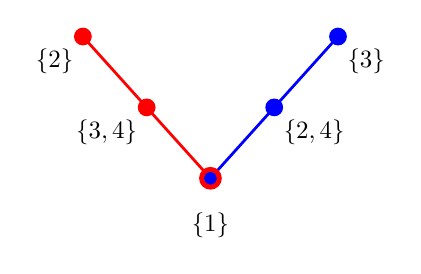
\begin{tikzpicture}[scale=0.90, transform shape, every path/.style={line width=1pt}]

% lines
\draw[red] (0,2)--(0.9,1)--(1.8,0);
\draw[blue]   (1.8,0)--(2.7,1)--(3.6,2);

% red context
\filldraw[fill=red, draw=red] (0,2) circle (3pt);
\node[left,yshift=-10pt] at (0,2) {$\{2\}$};

\filldraw[fill=red, draw=red] (0.9,1) circle (3pt);
\node[left,yshift=-10pt] at (0.9,1) {$\{3,4\}$};

% shared node c
\filldraw[fill=red, draw=red] (1.8,0) circle (4pt);
\filldraw[fill=blue,   draw=blue]   (1.8,0) circle (2pt);
\node[below,yshift=-10pt] at (1.8,0) {$\{1\}$};

% blue context
\filldraw[fill=blue, draw=blue] (2.7,1) circle (3pt);
\node[right,yshift=-10pt] at (2.7,1) {$\{2,4\}$};

\filldraw[fill=blue, draw=blue] (3.6,2) circle (3pt);
\node[right,yshift=-10pt] at (3.6,2) {$\{3\}$};

\end{tikzpicture}
\caption{Greechie diagram of the $L_{12}$ personnel-assessment
logic. Each line represents one context. The written-test context
(left) carries the observed categories $\{2\}$, $\{3,4\}$, and
$\{1\}$. The interview context (right) carries the observed
categories $\{3\}$, $\{2,4\}$, and $\{1\}$. The observed category
$\{1\}$ is the intertwining atom: it appears in both contexts
because the Star profile is identifiable regardless of which
instrument is chosen. The designation $L_{12}$ counts the
twelve elements of the pasted operational logic: each three-atom
Boolean block contributes $2^3=8$ elements, and the two blocks
share exactly $4$ elements (the intertwining atom $\{1\}$, its
block complement $\{2,3,4\}=\{3,4\}\cup\{2\}=\{2,4\}\cup\{3\}$
inside each block, together with $\emptyset$ and the unit), giving
$8+8-4=12$. The label $L_{12}$ does not refer to the full Boolean
algebra $2^{S_4}$, which has $16$ elements.}
\label{fig:L12}
\end{figure}

\subsection{What does the partition logic tell us?}

The partition logic $L_{12}$ (Fig.~\ref{fig:L12}) encodes a precise
tradeoff. By choosing the written test, the HR department can
distinguish type~2 from types~3 and~4, at the cost of being unable
to distinguish type~3 from type~4. By choosing the interview, it can
distinguish type~3 from types~2 and~4, but now type~2 and type~4 are
conflated. No single instrument resolves all four types. This is
complementarity: information about one aspect of the applicant comes
at the expense of information about the other. Yet every applicant
has a determinate type; the partition logic captures an epistemic
limitation of the observer, not an ontic indeterminacy of the system.

%--------------------------------------------------------------
\section{Scenario 2: Framing effects in public opinion surveys
(Pentagon logic)}
\label{sec:surveys}
%--------------------------------------------------------------

Our second scenario turns to political psychology. It shows how a
carefully idealized survey design with strong framing and order
effects can instantiate the cyclic structure of a pentagon partition
logic.

\subsection{What are the types?}

A political psychologist studies a population whose members differ
in their latent configuration of attitudes across five policy
domains. Rather than continuous attitude scales, suppose for
simplicity that the relevant attitudinal differences can be captured
by $n=11$ discrete respondent profiles, denoted
$S_{11}=\{1,2,\ldots,11\}$. The choice of $n=11$ is not arbitrary:
it is the minimum cardinality of a latent space that supports the
pentagon partition logic with all five contexts having three atoms
each and all five intertwining atoms being distinct subsets of $S$
~\cite[p.~267, Fig.~2]{wright:pent}. Smaller latent spaces force
identifications that collapse the cyclic structure. Each profile
specifies a particular pattern of beliefs about immigration,
healthcare, taxation, education, and defense spending. For example:
\begin{itemize}
\item Profile~1 might be a consistent moderate who holds centrist
views on all five issues.
\item Profile~7 might be a libertarian who favors minimal government
across all domains.
\item Profile~10 might be a hawk-dove who supports high defense
spending as well as generous social programs.
\end{itemize}
The eleven profiles are assumed exhaustive and mutually exclusive:
every respondent is exactly one profile.

\subsection{What are the contexts?}

The five policy issues define five survey contexts. In each context,
the respondent is asked a block of questions about one issue and the
response is classified into one of three opinion clusters, such as
supportive, moderate, and opposed. To idealize strong framing and
order effects~\cite{Moore2002}, suppose that the research design
treats each issue frame as a separate experimental condition. Each
respondent is assigned to one context only (between-subjects
design), so that cross-context joint responses are not taken as
observations of a single unchanged cognitive state.

The five contexts, adapted from the partition logic of the pentagon
~\cite{greechie-1974,wright:pent,svozil-2018-b}, are:
\begin{align}
C_1\;\text{(immigration)} &= \bigl\{\{1,2,3\},\;\{4,5,7,9,11\},\;
\{6,8,10\}\bigr\},
\notag\\
C_2\;\text{(healthcare)} &= \bigl\{\{6,8,10\},\;\{1,2,4,7,11\},\;
\{3,5,9\}\bigr\},
\notag\\
C_3\;\text{(taxation)} &= \bigl\{\{3,5,9\},\;\{1,4,6,10,11\},\;
\{2,7,8\}\bigr\},
\label{eq:pentagon}\\
C_4\;\text{(education)} &= \bigl\{\{2,7,8\},\;\{1,3,9,10,11\},\;
\{4,5,6\}\bigr\},
\notag\\
C_5\;\text{(defense)} &= \bigl\{\{4,5,6\},\;\{7,8,9,10,11\},\;
\{1,2,3\}\bigr\}.
\notag
\end{align}
Each context partitions all eleven profiles into three clusters.

\subsection{What are the intertwining atoms?}

Consider contexts $C_1$ and $C_2$. The atom $\{6,8,10\}$ appears as
one cluster in both contexts. Substantively, this means that profiles
6, 8, and 10 happen to look the same under the immigration frame and
under the healthcare frame. The cluster $\{6,8,10\}$ is an
intertwining atom precisely because the same subset of latent
profiles is produced by two different observational contexts.

The five intertwining atoms, one per adjacent pair of contexts, form
the outer vertices of the pentagon diagram (Fig.~\ref{fig:pentagon}):
\[
\{1,2,3\},\quad
\{6,8,10\},\quad
\{3,5,9\},\quad
\{2,7,8\},\quad
\{4,5,6\}.
\]
Formally, the five cyclically intertwined contexts form a
pentagon/pentagram logic~\cite[p.~267, Fig.~2]{wright:pent}
supporting eleven intended point-evaluation states. Constructing the
five contexts from the occurrences of value~$1$ in the corresponding
point states yields the partition logic
\begin{equation}
\begin{aligned}
&\{
 \{ \{ 1,2,3\} ,\{ 4,5,7,9,11\} ,\{ 6,8,10\} \} ,\\
&\{ \{ 6,8,10\} ,\{ 1,2,4,7,11\} ,\{ 3,5,9\} \} ,\\
&\{ \{ 3,5,9\} ,\{ 1,4,6,10,11\} ,\{ 2,7,8\} \} ,\\
&\{ \{ 2,7,8\} ,\{ 1,3,9,10,11\} ,\{ 4,5,6\} \} ,\\
&\{ \{ 4,5,6\} ,\{ 7,8,9,10,11\} ,\{ 1,2,3\} \}
\}.
\end{aligned}
\label{2018-e-plpentagon}
\end{equation}

\begin{figure}[t]
\centering
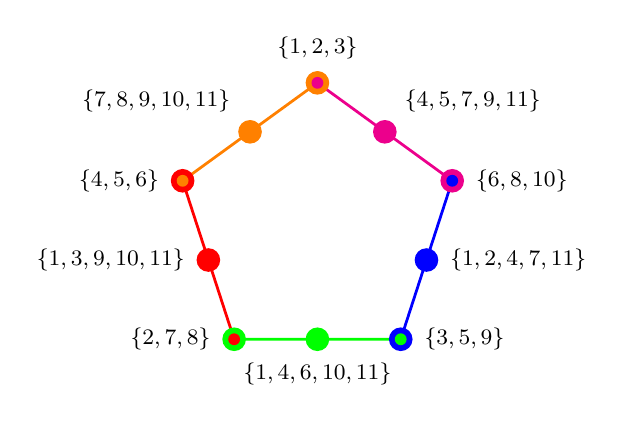
\begin{tikzpicture}  [scale=0.3]

\newdimen\ms
\ms=0.05cm

\tikzstyle{every path}=[line width=1pt]

\tikzstyle{c3}=[circle,inner sep={\ms/8},minimum size=6*\ms]
\tikzstyle{c2}=[circle,inner sep={\ms/8},minimum size=3*\ms]
\tikzstyle{c1}=[circle,inner sep={\ms/8},minimum size=0.8*\ms]

\newdimen\R
\R=6cm

\path
  ({90 + 0 * 360 /5}:\R      ) coordinate(1)
  ({90 + 36 + 0 * 360 /5}:{\R * sqrt((25+10*sqrt(5))/(50+10*sqrt(5)))}      ) coordinate(2)
  ({90 + 1 * 360 /5}:\R   ) coordinate(3)
  ({90 + 36 + 1 * 360 /5}:{\R * sqrt((25+10*sqrt(5))/(50+10*sqrt(5)))}   ) coordinate(4)
  ({90 + 2 * 360 /5}:\R  ) coordinate(5)
  ({90 + 36 + 2 * 360 /5}:{\R * sqrt((25+10*sqrt(5))/(50+10*sqrt(5)))}  ) coordinate(6)
  ({90 + 3 * 360 /5}:\R  ) coordinate(7)
  ({90 + 36 + 3 * 360 /5}:{\R * sqrt((25+10*sqrt(5))/(50+10*sqrt(5)))}  ) coordinate(8)
  ({90 + 4 * 360 /5}:\R     ) coordinate(9)
  ({90 + 36 + 4 * 360 /5}:{\R * sqrt((25+10*sqrt(5))/(50+10*sqrt(5)))}     ) coordinate(10)
;

\draw [color=orange] (1) -- (2) -- (3);
\draw [color=red] (3) -- (4) -- (5);
\draw[color=green] (5) -- (6) -- (7);
\draw [color=blue] (7) -- (8) -- (9);
\draw [color=magenta] (9) -- (10) -- (1);

\draw (1) coordinate[c3,fill=orange,label=90:{\footnotesize $\{ 1,2,3\} $}];
\draw (1) coordinate[c2,fill=magenta];

\draw (2) coordinate[c3,fill=orange,label={above left:\footnotesize $\{ 7,8,9,10,11\}$}];

\draw (3) coordinate[c3,fill=red,label={left:\footnotesize $\{ 4,5,6\} $}];
\draw (3) coordinate[c2,fill=orange];

\draw (4) coordinate[c3,fill=red,label={left:\footnotesize $\{ 1,3,9,10,11\}$}];

\draw (5) coordinate[c3,fill=green,label={left:\footnotesize $\{ 2,7,8\} $}];
\draw (5) coordinate[c2,fill=red];

\draw (6) coordinate[c3,fill=green,label={below:\footnotesize $\{ 1,4,6,10,11\} $}];

\draw (7) coordinate[c3,fill=blue,label={right:\footnotesize $\{ 3,5,9\}$}];
\draw (7) coordinate[c2,fill=green];

\draw (8) coordinate[c3,fill=blue,label={right:\footnotesize $\{ 1,2,4,7,11\}$}];

\draw (9) coordinate[c3,fill=magenta,label={right:\footnotesize $\{ 6,8,10\}$}];
\draw (9) coordinate[c2,fill=blue];

\draw (10) coordinate[c3,fill=magenta,label={above right:\footnotesize $\{ 4,5,7,9,11\}$}];

\end{tikzpicture}
\caption{Pentagon survey logic. Each color corresponds to one
survey context. Adjacent contexts share exactly one atom, producing
the cyclic pentagon structure. The construction is an idealized
experimental design for strong framing effects, not a claim that
ordinary multi-issue surveys are impossible.}
\label{fig:pentagon}
\end{figure}

\subsection{Why the pentagon structure matters: classical vs.\ quantum-like bounds}
\label{sec:pentagon-bounds}

Each intertwining atom is a subset of the eleven profiles. The
classical probability that a randomly drawn respondent falls in any
one of these subsets is simply the fraction of the population
belonging to the corresponding profiles. The key constraint is that
the five intertwining-atom subsets overlap in a restricted way:
each latent profile belongs to at most two of the five intertwining
atoms. Therefore, for every point state,
\[
\sum_{j=1}^{5}\chi_{A_j}(s)\leq 2,
\]
where $A_j$ denotes the $j$th intertwining atom. Taking the
expectation over any probability distribution on $S_{11}$ yields
\begin{equation}
\sum_{j=1}^{5} P(A_j) \leq 2.
\label{eq:classical_bound}
\end{equation}
This is the KCBS-type noncontextual bound for a five-cycle
exclusivity structure~\cite{Klyachko-2008,Bub-2009}. In the
between-subjects design proposed here, each $P(A_j)$ is estimated
as the marginal frequency with which respondents in the appropriate
arm fall into the cluster $A_j$, so that no respondent contributes
to two adjacent $A_j$'s simultaneously. No matter how the population
is distributed across the eleven profiles, the total
intertwining-atom weight cannot exceed~2.

If, however, the respondents' cognitive states are modeled by
vectors in a Hilbert space, as in quantum-cognition models
~\cite{Busemeyer2012}, then probabilities of the corresponding
five cyclic events can obey Born's rule. Under a suitable faithful
orthogonal representation of the five-cycle exclusivity structure,
one obtains the Lovasz-theta value
\begin{equation}
\sum_{j=1}^{5} P(A_j) \leq \sqrt{5}
\approx 2.236.
\label{eq:quantum_bound}
\end{equation}
This is about a twelve percent increase over the classical bound. A
survey experiment that implements the pentagon exclusivity structure
and finds aggregate intertwining-atom probabilities exceeding~2
would falsify the classical latent-partition model and motivate a
nonclassical, quantum-like cognitive model. Conversely, satisfaction
of the classical bound would support the more parsimonious
value-definite interpretation.

\paragraph{Caveats for the empirical test.}
Because the design is between-subjects, each intertwining atom
$A_j$ is in fact estimated from two distinct experimental arms (the
two adjacent contexts of which it is an atom). For the KCBS bound
to apply as written, an auxiliary \emph{marginal-consistency} or
\emph{no-disturbance} condition must hold: the estimated frequency
of $A_j$ must agree, within sampling error, between the two arms.
A failure of this condition---which is itself an empirically
checkable hypothesis---is a generic alternative explanation for any
apparent violation of~\eqref{eq:classical_bound}, distinct from
quantum cognition. Two further alternative explanations must also
be controlled for: (i)~\emph{selection effects}, including
framing-induced differential non-response and panel attrition, which
can mimic structure-violating frequencies without any cognitive
non-classicality; and (ii)~\emph{coarsening leakage}, in which the
three-cluster classification of one frame implicitly absorbs
information about other issues through correlated item wording,
breaking the assumed independence of contexts. A genuine empirical
case for quantum-cognitive structure thus requires ruling out, in
addition to~\eqref{eq:classical_bound}, these classical pathways to
apparent bound violation.

%--------------------------------------------------------------
\section{Scenario 3: Diagnostic complementarity in clinical psychology
(Triangle logic)}
\label{sec:clinical}
%--------------------------------------------------------------

Our third scenario turns to clinical diagnostics. It shows how
cyclic interference between different psychological and physiological
assessment tools can instantiate a triangle partition logic. As in
Scenario~1, the forced-choice restriction is a deliberate
idealization: real multimethod assessment batteries do administer
several instruments to the same patient, and the literature on
disturbance effects between them is itself contested. Our purpose is
to identify the abstract structure that \emph{would} arise if the
cyclic disturbance pattern below held to a sufficient degree.

\subsection{What are the latent states?}

A clinical psychologist suspects that patients presenting with
generalized anxiety disorder fall into four latent diagnostic
subtypes differing along two dimensions: cognitive worry and
physiological arousal. These subtypes are:
\begin{itemize}
\item \textbf{Latent state $1$ (``Cognitive-somatic''):} High
cognitive worry and high physiological arousal.
\item \textbf{Latent state $2$ (``Cognitive-dominant''):} High
cognitive worry but low physiological arousal.
\item \textbf{Latent state $3$ (``Somatic-dominant''):} Low
cognitive worry but high physiological arousal.
\item \textbf{Latent state $4$ (``Subclinical''):} Moderate levels
of both worry and arousal that fall below salient clinical
thresholds on either dimension taken alone.
\end{itemize}
The set of latent states is $S=\{1,2,3,4\}$. Each patient is exactly
one subtype; the diagnostic challenge is that no single instrument
can identify all four.

\subsection{What are the three contexts?}

Three diagnostic instruments are available. Each resolves two of the
three clear subtypes $1,2,3$ as singleton observed categories while
conflating the remaining clear subtype with the elusive subtype~$4$.

\begin{itemize}
\item \textbf{Context $\mathcal{C}_A$ --- Self-report questionnaire.}
The patient completes a standardized inventory of worry-related
cognitions. Instrument~A picks up the cognitive dimension:
\[
\mathcal{C}_A=\{\{1\},\{2\},\{3,4\}\}.
\]

\item \textbf{Context $\mathcal{C}_B$ --- Behavioral observation.}
A clinician observes the patient during a structured social
interaction and rates visible signs such as gaze aversion, fidgeting,
tremor, and speech latency. Instrument~B picks up the behavioral
expression of anxiety:
\[
\mathcal{C}_B=\{\{2\},\{3\},\{1,4\}\}.
\]

\item \textbf{Context $\mathcal{C}_C$ --- Physiological stress test.}
The patient undergoes a standardized stress-induction protocol while
heart-rate variability and cortisol are recorded. Instrument~C picks
up the somatic dimension:
\[
\mathcal{C}_C=\{\{1\},\{3\},\{2,4\}\}.
\]
\end{itemize}

\begin{table*}[htb]
\caption{\label{tab:clinical}How the four latent diagnostic
subtypes map to observed categories under each of the three
instruments. Boldface marks singleton observed categories; plain text
marks conflated pairs.}
\begin{center}
\begin{tabular}{lccc}
\colrule
Latent state & $\mathcal{C}_A$ (Self-report) &
  $\mathcal{C}_B$ (Behavioral) & $\mathcal{C}_C$ (Physiological)\\
\colrule
$1$ (Cognitive-somatic)  & \textbf{severe cognitive}  & unremarkable
  & \textbf{severe physiological}\\
$2$ (Cognitive-dominant)  & \textbf{moderate cognitive} & \textbf{avoidant}
  & low physiological\\
$3$ (Somatic-dominant)  & low cognitive  & \textbf{tremorous}
  & \textbf{moderate physiological}\\
$4$ (Subclinical) & low cognitive  & unremarkable
  & low physiological\\
\colrule
\end{tabular}
\end{center}
\end{table*}

Table~\ref{tab:clinical} summarizes the mapping. The crucial pattern
is that $4$ never forms a singleton. Under every instrument it is
conflated with a different partner: with $3$ under~A, with $1$
under~B, and with $2$ under~C. It is the ``stealth'' subtype that
each instrument misses in a different way.

\subsection{Why only one instrument per session?}

The three instruments interfere with one another in a cyclic pattern
that, in the idealized model, prevents sequential administration
within a single diagnostic session:
\begin{enumerate}
\item \emph{A degrades B.} Completing the self-report questionnaire
induces introspective self-focus, which alters the patient's
spontaneous behavior in the subsequent social interaction
~\cite{Duval1972}.
\item \emph{B degrades C.} The social interaction of being observed
by a rater elevates baseline physiological arousal through
social-evaluative threat~\cite{Dickerson2004}.
\item \emph{C degrades A.} Undergoing a physiological stress-induction
protocol triggers mood-congruent recall and somatic focusing,
biasing subsequent self-reports~\cite{Bower1981}.
\end{enumerate}
These interferences are systematic disturbances that change the
patient's momentary state in ways relevant to the other instruments.
The clinician is then forced to choose one instrument per session.
This is a paradigm case of disturbance-based complementarity (C2 in
the taxonomy of Section~\ref{sec:intro}): the forced choice arises
from the interplay between instruments rather than from any
intrinsic limitation of any single instrument.

\subsection{What are the intertwining atoms?}

Each pair of contexts shares exactly one observed category
(Table~\ref{tab:intertwine_clinical}):
\begin{itemize}
\item $\{1\}$ is shared by $\mathcal{C}_A$ and $\mathcal{C}_C$.
Both the self-report questionnaire and the physiological stress test
single out the Cognitive-somatic subtype.
\item $\{2\}$ is shared by $\mathcal{C}_A$ and $\mathcal{C}_B$.
The Cognitive-dominant subtype is identifiable whether one reads the
patient's report or watches the patient's behavior.
\item $\{3\}$ is shared by $\mathcal{C}_B$ and $\mathcal{C}_C$.
The Somatic-dominant subtype appears through both visible tremor and
physiological reactivity.
\end{itemize}

\begin{table*}[htb]
\caption{\label{tab:intertwine_clinical}Intertwining atoms of the
triangle logic. Each row names a pair of contexts, the shared
observed category, and the clinical reason why the subtype is
identifiable under both instruments.}
\begin{center}
\begin{tabular}{lll}
\colrule
Context pair & Shared atom & Reason for identifiability\\
\colrule
$\mathcal{C}_A$--$\mathcal{C}_C$ & $\{1\}$ &
  Extreme on both worry and arousal\\
$\mathcal{C}_A$--$\mathcal{C}_B$ & $\{2\}$ &
  High worry shows in report and behavior\\
$\mathcal{C}_B$--$\mathcal{C}_C$ & $\{3\}$ &
  High arousal shows in behavior and physiology\\
\colrule
\end{tabular}
\end{center}
\end{table*}

These three intertwining atoms are the vertices of a triangle in the
Greechie diagram (Fig.~\ref{fig:triangle}). Each edge of the triangle
represents one context; the non-shared observed categories
$\{3,4\}$, $\{1,4\}$, and $\{2,4\}$ sit at the midpoints of the
edges. The result is Wright's triangle logic~\cite[Figure~2,
p.~900]{wright}; see also Ref.~\cite[Fig.~6, Example~8.2,
pp.~414,420,421]{dvur-pul-svo}.

\begin{figure}[t]
\centering
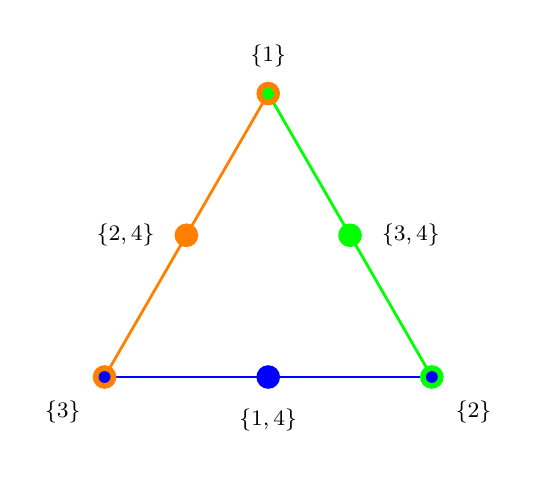
\begin{tikzpicture}  [scale=0.4]

\newdimen\ms
\ms=0.05cm

\tikzstyle{c3}=[circle,inner sep={\ms/8},minimum size=6*\ms]
\tikzstyle{c2}=[circle,inner sep={\ms/8},minimum size=3*\ms]
\tikzstyle{c1}=[circle,inner sep={\ms/8},minimum size=0.8*\ms]

\tikzstyle{every path}=[line width=1pt]

\newdimen\R
\R=6cm

\path
  ({90 + 0 * 360 /3}:\R      ) coordinate(1)
  ({90 + 1 * 360 /3}:\R   ) coordinate(3)
  ({90 + 2 * 360 /3}:\R  ) coordinate(5)
;

\draw [color=orange] (1) -- (3);
\draw [color=blue] (3) -- (5);
\draw [color=green] (5) -- (1);

\draw (1) coordinate[c3,fill=orange];
\draw (1) coordinate[c2,fill=green,label=90:\colorbox{white}{\footnotesize  $\{1\}$}];

\node[c3,fill=orange,label={left:\colorbox{white}{\footnotesize   $\{2,4\}$}}] at ( $ (1)!{1/2}!(3) $ ) (2) {};

\draw (3) coordinate[c3,fill=orange];
\draw (3) coordinate[c2,fill=blue,label=below left:{\footnotesize  \colorbox{white}{$\{3\}$}}];

\node[c3,fill=blue,label={below:{\footnotesize  \colorbox{white}{$\{1,4\}$}}}] at ( $ (3)!{1/2}!(5) $ ) (4) {};

\draw (5) coordinate[c3,fill=green];
\draw (5) coordinate[c2,fill=blue,label=below right:{\footnotesize   \colorbox{white}{$\{2\}$}}];

\node[c3,fill=green,label={right:\colorbox{white}{\footnotesize  $\{3,4\}$}}] at ( $ (5)!{1/2}!(1) $ ) (6) {};

\end{tikzpicture}
\caption{Greechie diagram of the triangle logic applied to clinical
diagnosis. Each edge represents one diagnostic context. The corner
vertices are the intertwining atoms: the singleton observed
categories, each identifiable under two adjacent instruments. The
midpoint vertices are the conflated observed categories, each merging
the subclinical subtype $4$ with a different partner. The six
observed categories form a non-Boolean pasted operational logic.
They are, of course, representable as subsets of the underlying
latent space \(S\); the non-Booleanity concerns the restricted
context-wise operations, not the nonexistence of an ambient Boolean
algebra.}
\label{fig:triangle}
\end{figure}

\subsection{The exotic probability weight: clinical interpretation}
\label{2026-pliss:exoticProbs}

Wright~\cite{wright:pent} (see also Ref.~\cite[Fig.~V]
{greechie-1974}) showed that cyclic logics with an odd number \(n\)
of intertwining atoms---including the triangle, pentagon, and
pentagram logics---support an ``exotic'' probability weight in
addition to their standard point-evaluation states. This weight
assigns value \(1/2\) to each cyclic intertwining vertex and lies
outside the classical convex hull. It is a probability weight on the
abstract pasted logic, not a probability measure induced by any
distribution over the intended latent social profiles.

To see this, consider the sum of the weights assigned to the \(n\)
cyclic intertwining atoms,
\[
S(\omega)=\sum_{i=1}^n\omega(v_i).
\]
Because these atoms are arranged in a cycle where each adjacent pair
\(\{v_i,v_{i+1}\}\) belongs to a common block, any valid weight must
satisfy
\[
\omega(v_i)+\omega(v_{i+1})\leq 1.
\]
For the exotic state \(\omega_{\rm ex}\), one has
\[
S(\omega_{\rm ex})=\frac n2.
\]
However, for any dispersion-free \(\{0,1\}\)-valued state on the
cycle, adjacent intertwining atoms cannot both receive value~\(1\).
On an odd cycle, the maximum number of non-adjacent vertices that can
receive value~\(1\) is \((n-1)/2\); hence
\[
S(\omega_c)\leq \frac{n-1}{2}
\]
for every classical deterministic state \(\omega_c\). Since every
state in the classical convex hull is a mixture of such deterministic
states, it also satisfies
\[
S(\omega_{\rm hull})\leq \frac{n-1}{2}.
\]
Because \(n/2>(n-1)/2\), the exotic state lies outside the classical
convex hull.

Wright motivated the empirical plausibility of such nonclassical
weights by giving a simple consumer-choice example. He wrote
\cite[p.~272]{wright:pent}:
\begin{quote}
``\dots suppose that there is a consumer who
has no strong opinions one way or the other about the products, so that
he is equally likely to say either yes or no to the first question, but
suppose, further, that he is embarrassed about saying no~\cite{smith1975} so that
if he says no to the first question, then he always says yes to the
second.''
\end{quote}
The point of Wright's example is not that the consumer has a fixed
pre-existing answer to all possible questions. Rather, the response
to a question is partly shaped by the local question context and by
the transition to the next admissible alternative. The resulting
probability assignment can be normalized within each context while
failing to arise from a single global distribution over pre-existing
answers.

The clinical example introduced in Section~\ref{sec:clinical}
provides a concrete interpretation of this exotic triangle weight.
Recall that the four latent diagnostic subtypes were denoted by
\(1,2,3,4\). Subtypes \(1,2,3\) are the three diagnostically salient
or ``clear'' presentations, while subtype~\(4\) is the subclinical or
masked presentation that is never identified as a singleton by any
one instrument. A diagnostic context means here one complete
diagnostic arrangement---for example, a self-report questionnaire, a
behavioral observation protocol, or a physiological stress test. Each
such arrangement partitions the same latent patient population into
the categories that this particular instrument can distinguish.

In the stylized triangle model, the three diagnostic contexts are
\[
\mathcal C_A=\{\{1\},\{2\},\{3,4\}\},
\]
\[
\mathcal C_B=\{\{2\},\{3\},\{1,4\}\},
\]
and
\[
\mathcal C_C=\{\{1\},\{3\},\{2,4\}\}.
\]
For instance, \(\mathcal C_A\) may be read as a self-report context:
it sharply distinguishes subtypes \(1\) and \(2\), but conflates
subtype \(3\) with the masked subtype~\(4\). Similarly,
\(\mathcal C_B\) may be read as a behavioral-observation context:
it sharply distinguishes subtypes \(2\) and \(3\), but conflates
subtype \(1\) with subtype~\(4\). Finally, \(\mathcal C_C\) may be
read as a physiological-stress context: it sharply distinguishes
subtypes \(1\) and \(3\), but conflates subtype \(2\) with
subtype~\(4\).

The resulting pasted logic has the form of a triangle. Its three
cyclic intertwining atoms are the singleton diagnostic categories
\[
\{1\},\qquad \{2\},\qquad \{3\}.
\]
They are called intertwining atoms because each of them occurs in
two different diagnostic contexts: \(\{1\}\) occurs in
\(\mathcal C_A\) and \(\mathcal C_C\), \(\{2\}\) occurs in
\(\mathcal C_A\) and \(\mathcal C_B\), and \(\{3\}\) occurs in
\(\mathcal C_B\) and \(\mathcal C_C\). The remaining atoms
\(\{3,4\}\), \(\{1,4\}\), and \(\{2,4\}\) are not shared between
contexts. They are context-specific conflations of one clear subtype
with the masked subtype~\(4\).

The exotic triangle weight assigns
\[
P(\{1\})=P(\{2\})=P(\{3\})=\frac12
\]
to the three singleton intertwining atoms and assigns probability
zero to the three non-shared atoms:
\[
P(\{3,4\})=P(\{1,4\})=P(\{2,4\})=0.
\]
This is a valid probability weight on the abstract pasted triangle
logic, because each diagnostic context is separately normalized:
\[
\mathcal C_A:\quad
P(\{1\})+P(\{2\})+P(\{3,4\})
=
\frac12+\frac12+0=1,
\]
\[
\mathcal C_B:\quad
P(\{2\})+P(\{3\})+P(\{1,4\})
=
\frac12+\frac12+0=1,
\]
and
\[
\mathcal C_C:\quad
P(\{1\})+P(\{3\})+P(\{2,4\})
=
\frac12+\frac12+0=1.
\]
Thus each instrument, considered by itself, yields an ordinary
normalized probability distribution over its three observed
categories.

What fails is the existence of a single underlying prevalence
distribution over the four intended latent diagnostic subtypes.
Suppose the population were described by fixed prevalences
\[
(\lambda_1,\lambda_2,\lambda_3,\lambda_4),
\qquad
\lambda_i\geq 0,\qquad
\sum_i\lambda_i=1.
\]
Then the probabilities of the three singleton categories would have
to be
\[
P(\{1\})=\lambda_1,\qquad
P(\{2\})=\lambda_2,\qquad
P(\{3\})=\lambda_3.
\]
Consequently,
\[
P(\{1\})+P(\{2\})+P(\{3\})
=
\lambda_1+\lambda_2+\lambda_3
\leq 1.
\]
The exotic triangle weight instead gives
\[
P(\{1\})+P(\{2\})+P(\{3\})
=
\frac32,
\]
which violates this classical latent-prevalence bound. Equivalently,
it would require
\[
\lambda_1=\lambda_2=\lambda_3=\frac12,
\]
which already sums to \(3/2\), before any probability is assigned to
subtype~\(4\).

The clinical interpretation must therefore be stated carefully. The
exotic weight does not describe an ordinary population in which each
patient has one fixed diagnostic subtype drawn from
\(\{1,2,3,4\}\). Rather, it describes a context-dependent diagnostic
response pattern. In each diagnostic arrangement, two singleton
categories are available as sharp classifications, and the population
is split evenly between them. The remaining clear subtype is not
available as a singleton in that arrangement, because it is absorbed
into the context-specific conflated atom containing the masked
subtype~\(4\). Which pair of singleton classifications is available
depends on the context:
\[
\mathcal C_A \text{ makes } \{1\}\text{ and }\{2\}\text{ sharp},
\]
\[
\mathcal C_B \text{ makes } \{2\}\text{ and }\{3\}\text{ sharp},
\]
and
\[
\mathcal C_C \text{ makes } \{1\}\text{ and }\{3\}\text{ sharp}.
\]
The same population can therefore display marginal weight \(1/2\) on
each of the three singleton diagnoses when these marginals are
estimated in the appropriate context arms, even though no single
fixed prevalence distribution over the four latent subtypes can
reproduce those three marginals simultaneously.

In this sense, Wright's consumer example and the clinical triangle
have the same formal moral. The empirical responses are locally
well-defined and normalized within each question or diagnostic
context, but they need not be marginals of one global distribution
over pre-existing answers or pre-existing diagnostic types. If
empirical frequencies in a clinical study approximated the exotic
triangle weight, the classical latent-partition model would therefore
be inadequate.

There are, however, several possible interpretations of such a
finding. A quantum-cognition interpretation would say that diagnostic
profiles are not merely revealed by the instrument but are partly
constituted by the diagnostic context~\cite{Busemeyer2012}. A more
conservative interpretation would be that the experimental design has
failed to implement the intended triangle logic: the three arms may
sample different populations, the instruments may not realize the
assumed partitions, or marginal consistency across shared atoms may
fail~\cite{Garg1984}. Thus the exotic weight should not be treated as a realistic
default model of clinical diagnosis. It is better understood as a
sharp benchmark separating ordinary fixed-subtype prevalence models
from genuinely context-dependent diagnostic probability assignments.

%--------------------------------------------------------------
\section{Scenario 4: Espionage and relational encoding---a classical
contrast case}
\label{sec:espionage}
%--------------------------------------------------------------

Our fourth scenario plays a different role from the previous three.
Rather than instantiating yet another non-Boolean partition logic,
it provides a deliberate \emph{contrast case}: it isolates what can
already be achieved by classical common-cause models with shared
preparation and no quantum or otherwise nonclassical resource. The
scenario thereby clarifies what is, and is not, distinctive about
the previous three structures, and prepares the ground for the
maximally complementary auditing example of
Section~\ref{sec:org}. By modeling two spatially separated espionage
agents sharing a predefined codebook, we construct a classical
analogue of one aspect---and only one aspect---of the
Einstein--Podolsky--Rosen setup: separated perfect correlations
generated by common preparation.

\subsection{What are the types?}

An intelligence agency trains agent pairs using a protocol that
creates correlations between their cover stories. Each agent pair is
prepared in one of four coordination types:
\begin{itemize}
\item \textbf{Type~1 (``Mirror''):} Both agents memorize clean
financial records and clean personal histories. Code: $00$.
\item \textbf{Type~2 (``Split-A''):} Agent~A memorizes a clean
financial record but a fabricated personal history; Agent~B
memorizes the reverse. Code: $01$.
\item \textbf{Type~3 (``Split-B''):} The reverse of Split-A. Code:
$10$.
\item \textbf{Type~4 (``Contrast''):} Both agents memorize
fabricated financial records and fabricated personal histories.
Code: $11$.
\end{itemize}
The latent space is again $S_4=\{00,01,10,11\}$.

\subsection{What are the contexts?}

Upon capture, each agent faces one of two interrogation modes:
\begin{itemize}
\item \textbf{Financial background check (F):} The interrogator
examines only financial records. The response is the first digit of
the code.
\item \textbf{Personal history interview (H):} The interrogator
examines only personal history. The response is the second digit of
the code.
\end{itemize}
An agent subjected to one mode gives answers that are psychologically
activated in a way that contaminates a subsequent interrogation in a
different mode. Thus only one mode is applied per agent.

For Alice the two interrogation modes define the partitions
\begin{align}
C_F^{(A)} &= \{\{1,2\},\{3,4\}\}
\quad\text{(first digit)}, \notag\\
C_H^{(A)} &= \{\{1,3\},\{2,4\}\}
\quad\text{(second digit)}.
\label{eq:alice}
\end{align}
Bob has the analogous pair of contexts.

\subsection{Relational encoding and why it is local}

The agency prepares agent pairs with a probability distribution
supported only on the two types
\[
D=\{01,10\},
\]
as shown in Table~\ref{tab:relational}. The latent space remains
$S_4$, but the preparation distribution is concentrated on this
two-element subensemble. Thus $D$ is not a new logic but a selected
preparation inside the original four-state classical model.

\begin{table}[b]
\caption{\label{tab:relational}Relational encoding of cover
stories for agent pairs. Each entry is a two-digit code. The
subensemble $S$ selects types with equal digits; the subensemble
$D$ selects types with unequal digits.}
\begin{center}
\begin{tabular}{lcccc}
\colrule
Sample & Type 1 & Type 2 & Type 3 & Type 4\\
\colrule
$S$ (same)  & 00 &  --  &  --  & 11 \\
$D$ (different) &  --  & 01 & 10 &  --  \\
\colrule
\end{tabular}
\end{center}
\end{table}

The relational encoding guarantees that if both agents face the same
interrogation mode, their answers are always opposite. When Alice's
financial check yields clean, Bob's yields fabricated, and vice
versa. This perfect anticorrelation arises entirely from the shared
codebook, a classical common cause established before separation.

\subsection{What this scenario shows---and what it does not}

This example is EPR-like only in the weak sense of separated perfect
correlations generated by common preparation. It is \emph{not}
Bell-nonlocal and cannot violate a Bell inequality. Its purpose
within this paper is twofold. First, it emphasizes that correlation
without communication is not uniquely quantum: a classical
common-cause distribution over a small latent space already produces
separated perfect anticorrelations. Second, by exhibiting the
strongest possible classical correlations on this graph, it sets the
benchmark above which genuinely nonclassical phenomena must operate.
What is uniquely quantum is not correlation per se but the
violation of Bell-type linear constraints across multiple
mismatched-context combinations, which the present preparation
demonstrably does not produce. Readers familiar with this point may
read the scenario as a sanity check: any social-science
``quantum-like'' claim must be measured against what such classical
constructions already deliver.

\subsection{Social science significance}

This scenario models situations in which two separated actors produce
correlated behaviors through shared preparation rather than direct
communication:
\begin{itemize}
\item \textbf{Coordinated deception:} Espionage cover stories.
\item \textbf{Institutional scripts:} Employees trained in the same
corporate protocol independently produce consistent behaviors when
facing customers~\cite{Cyert1963}.
\item \textbf{Shared cultural schemas:} Individuals socialized in
the same culture give correlated responses about values and norms
because they internalized the same codebook during childhood
~\cite{bordieu-fu}.
\end{itemize}
In all cases, the correlations are local and classical. They lie
within the classical polytope associated with the common-cause model.

%--------------------------------------------------------------
\section{Scenario 5: Legal pluralism and overlapping jurisdictions}
\label{sec:legal}
%--------------------------------------------------------------

Our fifth scenario applies partition logics to comparative law. The
existence of multiple overlapping legal frameworks creates a formal
structure of complementarity: the same action may be classified
differently depending on which legal code is applied. This is the
clearest example of framing-based complementarity (C3 of
Section~\ref{sec:intro}): no disturbance is involved, and the
forced choice arises because adjudication takes place within one
forum at a time, not because the act of legal classification
physically alters the action.

\subsection{What are the types?}

In a legally pluralistic society---for example, a post-colonial
state where statutory law, customary law, and religious law coexist
~\cite{Merry1988,Griffiths1986}---a citizen's action can be
classified differently depending on the framework. Consider six
types of land-use action:
\begin{itemize}
\item $a_1$: Clearing forest for subsistence farming on ancestral
land.
\item $a_2$: Clearing forest for commercial logging on ancestral
land.
\item $a_3$: Building a house on communally held village land.
\item $a_4$: Building a commercial structure on communally held
village land.
\item $a_5$: Grazing livestock on a protected nature reserve.
\item $a_6$: Grazing livestock on privately owned pasture.
\end{itemize}
Each action is a determinate fact; the question is how it is
categorized by different legal codes.

\subsection{What are the contexts?}

Three legal codes, each classifying actions into three categories,
define three contexts:
\begin{itemize}
\item \textbf{Statutory environmental law ($C_{\text{stat}}$):}
Focuses on environmental impact:
\[
C_{\text{stat}}=\{\{a_1,a_2\},\{a_3,a_4\},\{a_5,a_6\}\}.
\]
\item \textbf{Customary law ($C_{\text{cust}}$):}
Focuses on ancestral rights and communal obligations:
\[
C_{\text{cust}}=\{\{a_1,a_3\},\{a_2,a_5\},\{a_4,a_6\}\}.
\]
\item \textbf{Religious law ($C_{\text{rel}}$):}
Focuses on stewardship obligations:
\[
C_{\text{rel}}=\{\{a_1,a_2\},\{a_3,a_5\},\{a_4,a_6\}\}.
\]
\end{itemize}

\begin{table}[b]
\caption{\label{tab:legal}Classification of six land-use actions
under three legal codes. Actions in the same cell of a given column
are indistinguishable under that code.}
\begin{center}
\begin{tabular}{lccc}
\colrule
Action & Statutory & Customary & Religious \\
\colrule
$a_1$ (subsist.\ clearing) & Prohibited & Permitted & Prohibited \\
$a_2$ (comm.\ logging)     & Prohibited & Restricted & Prohibited \\
$a_3$ (house on village)   & Restricted & Permitted & Permitted \\
$a_4$ (shop on village)    & Restricted & Neutral & Discouraged \\
$a_5$ (graze on reserve)   & Permitted  & Restricted & Permitted \\
$a_6$ (graze on private)   & Permitted  & Neutral & Discouraged \\
\colrule
\end{tabular}
\end{center}
\end{table}

\subsection{What are the intertwining atoms?}

Two atoms are shared:
\begin{itemize}
\item $\{a_1,a_2\}$ is an intertwining atom of $C_{\text{stat}}$
and $C_{\text{rel}}$: both statutory and religious law treat forest
clearing as a single prohibited class.
\item $\{a_4,a_6\}$ is an intertwining atom of $C_{\text{cust}}$
and $C_{\text{rel}}$: both customary and religious law place these
commercial or noncommunal uses in a separate category, although they
interpret the category differently.
\end{itemize}

\begin{figure}[t]
\centering
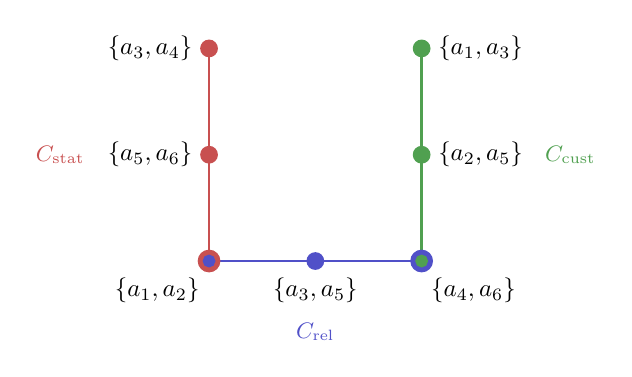
\begin{tikzpicture}[scale=0.90, transform shape, every path/.style={line width=1pt}]

\definecolor{statutory}{RGB}{200,80,80}
\definecolor{customary}{RGB}{80,160,80}
\definecolor{religious}{RGB}{80,80,200}

\draw[statutory] (0,3) -- (0,1.5) -- (0,0);
\draw[religious] (0,0) -- (1.5,0) -- (3,0);
\draw[customary] (3,0) -- (3,1.5) -- (3,3);

\filldraw[fill=statutory, draw=statutory] (0,3) circle (3pt);
\node[left, font=\normalsize] at (-0.1,3) {$\{a_3, a_4\}$};

\filldraw[fill=statutory, draw=statutory] (0,1.5) circle (3pt);
\node[left, font=\normalsize] at (-0.1,1.5) {$\{a_5, a_6\}$};

\filldraw[fill=statutory, draw=statutory] (0,0) circle (4pt);
\filldraw[fill=religious, draw=religious] (0,0) circle (2pt);
\node[below left, font=\normalsize] at (0,-0.1) {$\{a_1, a_2\}$};

\filldraw[fill=religious, draw=religious] (1.5,0) circle (3pt);
\node[below, font=\normalsize] at (1.5,-0.1) {$\{a_3, a_5\}$};

\filldraw[fill=religious, draw=religious] (3,0) circle (4pt);
\filldraw[fill=customary, draw=customary] (3,0) circle (2pt);
\node[below right, font=\normalsize] at (3,-0.1) {$\{a_4, a_6\}$};

\filldraw[fill=customary, draw=customary] (3,1.5) circle (3pt);
\node[right, font=\normalsize] at (3.1,1.5) {$\{a_2, a_5\}$};

\filldraw[fill=customary, draw=customary] (3,3) circle (3pt);
\node[right, font=\normalsize] at (3.1,3) {$\{a_1, a_3\}$};

\node[statutory, font=\small] at (-2.1,1.5) {$C_{\text{stat}}$};
\node[religious, font=\small] at (1.5,-1) {$C_{\text{rel}}$};
\node[customary, font=\small] at (5.1,1.5) {$C_{\text{cust}}$};

\end{tikzpicture}
\caption{Hypergraph of the legal-pluralism logic. Three legal codes
form three contexts. The corner vertices $\{a_1,a_2\}$ and
$\{a_4,a_6\}$ are intertwining atoms, each shared by two codes.
Other vertices represent groupings specific to one code. The
non-Boolean pasting captures the restricted operational structure of
forum-dependent classification; the full Boolean refinement over the
six action types still exists.}
\label{fig:legal}
\end{figure}

\subsection{What does the non-Boolean structure mean for legal practice?}

In practice, a land-use dispute is adjudicated under one legal
framework at a time: the choice of forum determines which distinctions
are drawn and which actions are conflated. Under statutory law,
subsistence clearing and commercial logging are treated identically;
customary law treats them differently. Under customary law, a house
and a shop on village land are different categories; under statutory
law both are merely restricted.

The non-Boolean pasted structure does not mean that no common
set-theoretic refinement exists. The six action types themselves
provide one. Rather, it means that no single legal forum among the
three available codes operationally applies all distinctions
simultaneously. Each code induces its own coarse graining, and legal
outcome depends on the selected forum. In this sense, forum choice is
analogous to context choice in a measurement procedure---a pure case
of framing-based complementarity without any disturbance dynamics.

%--------------------------------------------------------------
\section{Scenario 6: Organizational auditing with measurement
disturbance}
\label{sec:org}
%--------------------------------------------------------------

Our final scenario models organizational auditing. It serves two
purposes. First, it exhibits \emph{maximal} complementarity at the
partition-logic level: the two available audit contexts share no
intertwining atom, so the resulting pasted structure is just two
disjoint Boolean blocks sharing only $\emptyset$ and the unit. The
non-Booleanity is therefore trivial. What carries the substantive
content of the example is the second feature: the act of inspection
disturbs the corporation's internal state, so that this scenario is
the cleanest illustration of disturbance-based complementarity (C2)
in our taxonomy. We retain the label ``automaton'' only in the
informal sense that the contexts induce state transitions; a fully
formal automaton partition logic in the sense of Schaller and Svozil
~\cite{schaller-92,svozil-2001-eua} would specify a transition
function $\delta\colon S\times\{a,b\}\to S$ together with output
maps, which we sketch but do not develop in detail below.

\subsection{What are the types?}

A government regulatory agency must assess whether a corporation
complies with regulations. The corporation can be in one of four
internal organizational states, characterized by two binary dimensions:
\begin{itemize}
\item \textbf{Financial health:} Sound ($0$) vs. distressed ($1$).
\item \textbf{Operational compliance:} Compliant ($0$) vs.
non-compliant ($1$).
\end{itemize}
The four states are:
\begin{itemize}
\item $s_1=(0,0)$: Financially sound and operationally compliant.
\item $s_2=(0,1)$: Financially sound but operationally non-compliant.
\item $s_3=(1,0)$: Financially distressed but operationally compliant.
\item $s_4=(1,1)$: Financially distressed and operationally
non-compliant.
\end{itemize}
At a fixed time, each corporation is exactly one of these four states.

\subsection{What are the contexts?}

The auditor can probe the corporation by issuing one of two directives:
\begin{itemize}
\item \textbf{Financial audit (directive $a$):} The auditor requests
detailed financial records. The response reveals financial health
(the first digit), but preparing financial disclosures reallocates
organizational resources and may alter operational compliance.
The corresponding partition is
\[
C_a=\{\{s_1,s_2\},\{s_3,s_4\}\}.
\]
\item \textbf{Operational inspection (directive $b$):} The auditor
sends inspectors to the factory floor. The response reveals
operational compliance (the second digit), but the disruption of the
inspection may alter the financial state. The corresponding
partition is
\[
C_b=\{\{s_1,s_3\},\{s_2,s_4\}\}.
\]
\end{itemize}

\begin{figure}[t]
\centering
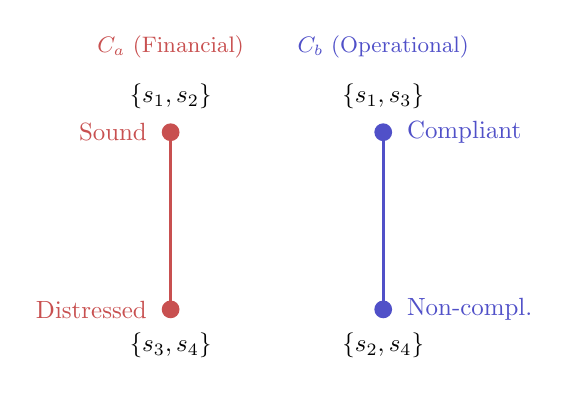
\begin{tikzpicture}[scale=0.90, transform shape, every path/.style={line width=1pt}]

\definecolor{financial}{RGB}{200,80,80}
\definecolor{operational}{RGB}{80,80,200}

\draw[financial] (0,0) -- (0,2.5);

\filldraw[fill=financial, draw=financial] (0,2.5) circle (3pt);
\node[above, font=\normalsize] at (0,2.7) {$\{s_1, s_2\}$};
\node[left, xshift=-10pt, font=\normalsize, financial] at (0.15,2.5) {Sound};

\filldraw[fill=financial, draw=financial] (0,0) circle (3pt);
\node[below, font=\normalsize] at (0,-0.2) {$\{s_3, s_4\}$};
\node[left, xshift=-10pt, font=\normalsize, financial] at (0.15,0) {Distressed};

\draw[operational] (3,0) -- (3,2.5);

\filldraw[fill=operational, draw=operational] (3,2.5) circle (3pt);
\node[above, font=\normalsize] at (3,2.7) {$\{s_1, s_3\}$};
\node[right, xshift=10pt, font=\normalsize, operational] at (2.85,2.5) {Compliant};

\filldraw[fill=operational, draw=operational] (3,0) circle (3pt);
\node[below, font=\normalsize] at (3,-0.2) {$\{s_2, s_4\}$};
\node[right, xshift=10pt, font=\normalsize, operational] at (2.85,0) {Non-compl.};

\node[financial, font=\small] at (0,3.7) {$C_a$ (Financial)};
\node[operational, font=\small] at (3,3.7) {$C_b$ (Operational)};

\end{tikzpicture}
\caption{Two complementary audit contexts for the four organizational
states. The financial audit partitions the state space by financial
health and conflates compliance status. The operational inspection
partitions the same state space by compliance status and conflates
financial health. The two partitions share no atoms, giving maximal
complementarity at the operational level.}
\label{fig:org_grid}
\end{figure}

\subsection{What are the intertwining atoms?}

In this scenario, the two partitions share no intertwining atoms:
\begin{align}
C_a &= \{\{s_1,s_2\},\{s_3,s_4\}\},
\notag\\
C_b &= \{\{s_1,s_3\},\{s_2,s_4\}\}.
\label{eq:org}
\end{align}
The set $\{s_1,s_2\}$ (sound) is not the same as
$\{s_1,s_3\}$ (compliant). Hence no atom appears in both contexts.
There is no organizational property in this two-context model that
can be ascertained regardless of audit type. This is maximal
complementarity in the operational sense---but, as noted above, it
is also a structurally trivial case at the level of the pasted
logic: with no intertwining atoms, the two Boolean blocks share only
$\emptyset$ and $S$, and the only operational ``constraint'' is the
forced choice between contexts.

\subsection{From two-context complementarity to automaton dynamics}
\label{sec:org-automaton}

What gives this example its substantive content is the
\emph{dynamics} induced by the audit directives. We now sketch the
additional automaton structure that would be needed to capture this
formally.

This formalization connects to Herbert Simon's concept of bounded
rationality~\cite{Simon1957}. An external regulator attempting to
understand an organization faces an irreducible limitation imposed by
the available probes. At a fixed time, the corporation's state can be
represented by an ordinary probability distribution over the four
Boolean states $(0,0),(0,1),(1,0),(1,1)$. The nonclassical feature of
the auditing model is not the absence of such a distribution, but the
fact that probing one coordinate may change the subsequent state of
the system.

Formally, the natural extension is a Mealy-style automaton over the
state space $S=\{s_1,s_2,s_3,s_4\}$ with input alphabet $\{a,b\}$,
output alphabet $\{0,1\}$, transition function $\delta\colon S\times
\{a,b\}\to S$, and output map $\lambda\colon S\times\{a,b\}\to\{0,1\}$
defined so that $\lambda(s,a)$ returns the first coordinate of $s$
and $\lambda(s,b)$ the second. The disturbance is encoded in
$\delta$: a financial audit may flip the operational coordinate
(``$\delta(s,a)$ may differ from $s$ in the second digit''), and an
operational inspection may flip the financial coordinate. The
two-context partition logic above is then the snapshot view at any
fixed time; the full empirical content emerges from sequences of
directives.

This is the measurement-disturbance problem of quantum mechanics
realized here by a completely classical mechanism: the audit process
itself consumes resources and changes the organization. A systematic
development of the resulting automaton partition logic, including
the order effects across sequences of directives and the
non-commutativity of $a$ and $b$ at the level of observed outputs,
follows the template of Refs.~\cite{schaller-92,svozil-2001-eua} and
is left for future work. The point we wish to make here is only that
this scenario clearly exhibits disturbance-based complementarity (C2)
even though its instantaneous partition logic (C1) is trivial.

%--------------------------------------------------------------
\section{Discussion: Probability models and quantum cognition}
\label{sec:discussion}
%--------------------------------------------------------------

The preceding examples show how partition logics can be instantiated
across several social-science domains. We now return to the
probability question. The central lesson is that operational
complementarity, logical non-Booleanity, and nonclassical
probability are distinct notions.

\subsection{Summary of the layered interpretation}

All six scenarios share a common formal skeleton: a finite latent
state space $S$, together with several partitions of $S$ representing
available observational contexts. Three levels must be kept separate:

\begin{enumerate}
\item \textbf{The latent Boolean space.}
At the ontological level of the model, all latent states are ordinary
elements of $S$, and all subsets belong to the Boolean algebra
$2^S$. In this sense the model is fully value-definite.

\item \textbf{The operational pasted logic.}
The observer does not have operational access to all distinctions in
$2^S$. Only the atoms belonging to available contexts are observed,
and only context-wise Boolean operations are operationally licensed.
The resulting pasted event structure can be non-Boolean even though
it is represented by subsets of $S$.

\item \textbf{Probability models.}
Classical probabilities arise from distributions over $S$ and hence
from convex mixtures of point-evaluation states. Abstract two-valued
weights, Born-rule probabilities, and exotic fractional weights may
also be studied on the same or related pasted structures, but they
need not correspond to distributions over the intended latent social
profiles.
\end{enumerate}

Crosscutting these three levels are the three notions of
complementarity (C1)--(C3) introduced in Section~\ref{sec:intro}.
Logical non-Booleanity (C1) belongs to level~2; disturbance-based
complementarity (C2) is a dynamical statement that goes beyond a
fixed-time partition logic and lives most naturally at the
automaton/transition level (Section~\ref{sec:org-automaton});
framing-based complementarity (C3) typically belongs to level~1, in
that different contexts impose different coarse-grainings of an
unchanged latent space. The six scenarios are therefore not
interchangeable instantiations of a single phenomenon: they
illustrate different combinations of (C1)--(C3) on top of the same
formal skeleton.

\subsection{Why this matters for social science}

\paragraph{The resource determines the probability theory.}
The same exclusivity graph can be realized by a classical urn, a
finite automaton, a social-science black box, or a quantum system.
A Wright urn or a determinate latent-profile model yields classical
probabilities. A quantum system can yield probabilities in a
Lovasz-theta-type set. An abstract odd-cycle logic may also support
exotic fractional weights. The graph alone does not settle the
matter; the realizing resource does.

\paragraph{Complementarity does not imply contextuality.}
All six scenarios feature complementarity: the inability to perform
all measurements simultaneously on an unchanged system. Yet the
intended social systems remain value-definite. The applicant has a
competence profile, the patient has a subtype, the legal action is a
determinate action, and the organization has an internal state. These
partition models therefore illustrate that complementarity does not
imply Kochen--Specker contextuality~\cite{kochen1}. The relevant
partition logics possess sufficiently many point-evaluation states to
separate the intended latent profiles. Their non-Booleanity is
operational and epistemic, not ontic.

\paragraph{Testable predictions and their alternative explanations.}
The distinction becomes empirically important when probabilities are
measured. Consider a social-measurement experiment implementing a
five-cycle exclusivity structure. If the observed probabilities of
the five cyclic events satisfy the classical bound~\eqref{eq:classical_bound},
then a latent partition model remains viable. If they exceed the
classical bound but remain within the quantum-like bound
~\eqref{eq:quantum_bound}, then a quantum-cognition model gains
support. If they violate even the quantum-like bound, then either the
intended exclusivity structure has not been implemented or a still
different probabilistic model is required.

This three-way contrast (classical / quantum-like / beyond) is what
gives the framework its empirical content, but it must be guarded
against several standard alternative explanations for any apparent
violation of the classical bound, none of which require any
quantum-cognitive ontology:
\begin{enumerate}
\item \emph{Failure of marginal consistency (no-disturbance).}
In a between-subjects design, each intertwining atom is estimated
twice, once in each of the two adjacent context arms. A discrepancy
between the two estimates breaks the inequality derivation
of~\eqref{eq:classical_bound} and can produce apparent violations
without any nonclassical resource.
\item \emph{Selection effects.}
Framing-induced differential non-response, panel attrition, and
self-selection into arms can bias marginal frequencies. A pentagon
experiment in which respondents in the ``defense'' arm differ
systematically in baseline attitudes from those in the
``immigration'' arm cannot be analyzed as if all arms sample the
same latent population.
\item \emph{Frame leakage and contextual coarsening.}
If the wording of items in one frame implicitly references content
relevant to another frame, the assumed independence of contexts
breaks down. The same applies if the three-cluster classification of
responses is itself data-dependent rather than fixed in advance.
\item \emph{Mis-specified exclusivity structure.}
The graph $G$ assumed in the analysis must match the operationally
realized exclusivity relations. If two atoms claimed to belong to a
common context in fact correspond to non-exclusive empirical
events, the classical bound does not apply.
\end{enumerate}
A genuine empirical case for quantum-cognitive structure thus
requires not only an apparent bound violation but also a positive
demonstration that none of (1)--(4) is responsible. Pre-registered
designs that include explicit marginal-consistency checks, balanced
randomization, and pre-specified clustering rules are essential for
this purpose.

\paragraph{Ontological or measurement-induced uncertainty.}
So far, we have presumed that uncertainty and complementarity arise
because underlying properties are latent and observational means are
limited. This is a purely epistemic stance. One may instead ask
whether some social or cognitive properties are not merely hidden but
partly constituted by the act of measurement. Such behavior would
require a stronger formalism than classical partition logic, perhaps
involving Kochen--Specker-type contextuality~\cite{kochen1} or
dynamical models in which the act of measurement changes the state.
The organizational audit example already points in this direction:
its automaton aspect arises not from the absence of latent states but
from state transitions induced by probes.

\paragraph{Non-uniform hypergraphs and varying block sizes.}
As noted in Section~\ref{sec:prelim-gr}, the six scenarios presented
here use uniform hypergraphs: every context yields the same number of
mutually exclusive observed categories. In the social sciences,
however, there is no a priori reason for such regularity. A job
interview might distinguish three outcome categories while a
psychometric test distinguishes five. Formally, the blocks of the
partition logic may be Boolean algebras of different orders
~\cite{greechie:71}. This does not undermine the basic framework:
the admissibility axioms of additivity and normalization apply block
by block. What does require additional work is the analysis of
faithful orthogonal representations and the associated probability
polytopes for such non-uniform structures. That systematic study is
left for future work.

%--------------------------------------------------------------
\section{Conclusion}
\label{sec:conclusion}
%--------------------------------------------------------------

We have shown how partition logics---non-Boolean operational
structures originally developed in the foundations of quantum
mechanics, generalized urn models, and automata theory
~\cite{svozil-2001-eua}---can be instantiated in five stylized
social-science scenarios, with a sixth (Section~\ref{sec:espionage})
included as a deliberate classical contrast case. In each
non-contrast scenario, a finite set of underlying types is
partitioned by multiple incompatible observational procedures:
assessment instruments, survey frames, diagnostic tests, legal
codes, or audit directives. The resulting structures exhibit
complementarity in one or more of the three senses (C1)--(C3)
distinguished in Section~\ref{sec:intro}: no single procedure
reveals all relevant distinctions. Yet every system has a fully
determinate type. The limitation is epistemic and operational, not
ontic.

The social-science scenarios therefore occupy a position between
ordinary Boolean description and genuinely quantum contextuality.
They have non-Boolean operational logics and complementarity, but
retain full value definiteness~\cite{svozil-2018-b}. This
demonstrates concretely that complementarity does not imply
Kochen--Specker contextuality. A pasted operational event structure
may fail to be Boolean under its restricted operations even though it
is represented inside an ambient Boolean algebra of latent states.

At the same time, the mathematical fact that many such structures
also admit quantum-like or exotic probability weights opens a door to
empirical testing. If human cognitive or social systems produce
probability distributions that violate the classical convex-hull
bounds but respect quantum-like or other admissible bounds---and the
classical alternative explanations enumerated in
Section~\ref{sec:discussion} have been ruled out---the
partition-logic framework provides the language in which to formulate
and test this hypothesis. Conversely, if the classical bounds are
respected, the partition logic with its convex hull of
point-evaluation states provides a complete and parsimonious account
of the observed complementarity---no quantum formalism is required.

The development of experiments that probe these questions---for
instance, large-scale pre-registered surveys with carefully designed
pentagon structures, including explicit marginal-consistency checks,
or clinical assessment batteries with triangle-logic
configurations---is a promising direction for future work at the
intersection of formal logic, quantum foundations, and social
science methodology.

\section*{Acknowledgments}
This research was funded in whole or in part by the \textit{Austrian Science Fund (FWF)} [Grant \href{https://doi.org/10.55776/PIN5424624}{DOI:10.55776/PIN5424624}].
The author acknowledges TU Wien Bibliothek for financial support through its Open Access Funding Programme.

\makeatletter
\renewcommand{\bibsection}{%
  \section*{References}%
  \@mkboth{REFERENCES}{REFERENCES}%
}
\makeatother

%\bibliographystyle{apacite}
%\bibliography{svozil}


\begin{thebibliography}{}

\bibitem [\protect \citeauthoryear {%
Aerts%
}{%
Aerts%
}{%
{\protect \APACyear {2024}}%
}]{%
aerts2024quantum}
\APACinsertmetastar {%
aerts2024quantum}%
\begin{APACrefauthors}%
Aerts, D.%
\end{APACrefauthors}%
\unskip\
\newblock
\APACrefYearMonthDay{2024}{}{}.
\newblock
{\BBOQ}\APACrefatitle {Quantum Theory and Its Puzzles: Not Wave-Particles but
  Language-Particles} {Quantum theory and its puzzles: Not wave-particles but
  language-particles}.{\BBCQ}
\newblock
\APACjournalVolNumPages{Medium.com}{}{}{1--12}.
\newblock
\begin{APACrefURL}
  \url{https://medium.com/quantum-physics/quantum-theory-and-its-puzzles-not-wave-particles-but-language-particles-9bac94ffb069}
  \end{APACrefURL}
\PrintBackRefs{\CurrentBib}

\bibitem [\protect \citeauthoryear {%
Aerts%
\ \BBA {} Aerts%
}{%
Aerts%
\ \BBA {} Aerts%
}{%
{\protect \APACyear {1995}}%
}]{%
aerts1995applications}
\APACinsertmetastar {%
aerts1995applications}%
\begin{APACrefauthors}%
Aerts, D.%
\BCBT {}\ \BBA {} Aerts, S.%
\end{APACrefauthors}%
\unskip\
\newblock
\APACrefYearMonthDay{1995}{}{}.
\newblock
{\BBOQ}\APACrefatitle {Applications of quantum statistics in psychological
  studies of decision processes} {Applications of quantum statistics in
  psychological studies of decision processes}.{\BBCQ}
\newblock
\APACjournalVolNumPages{Foundations of Science}{1}{1}{85--97}.
\newblock
\begin{APACrefURL} \url{https://doi.org/10.1007/BF00208726} \end{APACrefURL}
\newblock
\begin{APACrefDOI} \doi{10.1007/BF00208726} \end{APACrefDOI}
\PrintBackRefs{\CurrentBib}

\bibitem [\protect \citeauthoryear {%
Aerts%
, Aerts%
\BCBL {}\ \BBA {} Gabora%
}{%
Aerts%
\ \protect \BOthers {.}}{%
{\protect \APACyear {2009}}%
}]{%
aerts2009experimental}
\APACinsertmetastar {%
aerts2009experimental}%
\begin{APACrefauthors}%
Aerts, D.%
, Aerts, S.%
\BCBL {}\ \BBA {} Gabora, L.%
\end{APACrefauthors}%
\unskip\
\newblock
\APACrefYearMonthDay{2009}{}{}.
\newblock
{\BBOQ}\APACrefatitle {Experimental Evidence for Quantum Structure in
  Cognition} {Experimental evidence for quantum structure in cognition}.{\BBCQ}
\newblock
\BIn{} P.~Bruza, D.~Sofge, W.~Lawless, K.~van Rijsbergen\BCBL {}\ \BBA {}
  M.~Klusch\ (\BEDS), \APACrefbtitle {Quantum Interaction} {Quantum
  interaction}\ (\BPGS\ 59--70).
\newblock
\APACaddressPublisher{Cham}{Springer}.
\newblock
\begin{APACrefURL} \url{https://doi.org/10.1007/978-3-642-00834-4_7}
  \end{APACrefURL}
\newblock
\begin{APACrefDOI} \doi{10.1007/978-3-642-00834-4_7} \end{APACrefDOI}
\PrintBackRefs{\CurrentBib}

\bibitem [\protect \citeauthoryear {%
Aerts%
\ \BBA {} Aerts~Argu\"{e}lles%
}{%
Aerts%
\ \BBA {} Aerts~Argu\"{e}lles%
}{%
{\protect \APACyear {2022}}%
}]{%
aerts2022human}
\APACinsertmetastar {%
aerts2022human}%
\begin{APACrefauthors}%
Aerts, D.%
\BCBT {}\ \BBA {} Aerts~Argu\"{e}lles, J.%
\end{APACrefauthors}%
\unskip\
\newblock
\APACrefYearMonthDay{2022}{}{}.
\newblock
{\BBOQ}\APACrefatitle {Human Perception as a Phenomenon of Quantization} {Human
  perception as a phenomenon of quantization}.{\BBCQ}
\newblock
\APACjournalVolNumPages{Entropy}{24}{9}{1207}.
\newblock
\begin{APACrefURL} \url{https://doi.org/10.3390/e24091207} \end{APACrefURL}
\newblock
\begin{APACrefDOI} \doi{10.3390/e24091207} \end{APACrefDOI}
\PrintBackRefs{\CurrentBib}

\bibitem [\protect \citeauthoryear {%
Aerts%
, Aerts~Argu\"{e}lles%
, Beltran%
\BCBL {}\ \BBA {} Sozzo%
}{%
Aerts%
\ \protect \BOthers {.}}{%
{\protect \APACyear {2023}}%
}]{%
aerts2023thermodynamics}
\APACinsertmetastar {%
aerts2023thermodynamics}%
\begin{APACrefauthors}%
Aerts, D.%
, Aerts~Argu\"{e}lles, J.%
, Beltran, L.%
\BCBL {}\ \BBA {} Sozzo, S.%
\end{APACrefauthors}%
\unskip\
\newblock
\APACrefYearMonthDay{2023}{}{}.
\newblock
{\BBOQ}\APACrefatitle {Development of a Thermodynamics of Human Cognition and
  Human Culture} {Development of a thermodynamics of human cognition and human
  culture}.{\BBCQ}
\newblock
\APACjournalVolNumPages{Philosophical Transactions of the Royal Society
  A}{381}{2256}{20220378}.
\newblock
\begin{APACrefURL} \url{https://doi.org/10.1098/rsta.2022.0378}
  \end{APACrefURL}
\newblock
\begin{APACrefDOI} \doi{10.1098/rsta.2022.0378} \end{APACrefDOI}
\PrintBackRefs{\CurrentBib}

\bibitem [\protect \citeauthoryear {%
Aerts%
, Aerts~Argu\"{e}lles%
\BCBL {}\ \BBA {} Sozzo%
}{%
Aerts%
\ \protect \BOthers {.}}{%
{\protect \APACyear {2025}}%
}]{%
aerts2025quantum}
\APACinsertmetastar {%
aerts2025quantum}%
\begin{APACrefauthors}%
Aerts, D.%
, Aerts~Argu\"{e}lles, J.%
\BCBL {}\ \BBA {} Sozzo, S.%
\end{APACrefauthors}%
\unskip\
\newblock
\APACrefYearMonthDay{2025}{}{}.
\newblock
\APACrefbtitle {Quantum Measurement, Entanglement and the Warping Mechanism of
  Human Perception.} {Quantum measurement, entanglement and the warping
  mechanism of human perception.}
\newblock
\begin{APACrefURL} \url{https://doi.org/10.48550/arXiv.2505.00777}
  \end{APACrefURL}
\newblock
\begin{APACrefDOI} \doi{10.48550/arXiv.2505.00777} \end{APACrefDOI}
\PrintBackRefs{\CurrentBib}

\bibitem [\protect \citeauthoryear {%
Aerts%
, D'Hooghe%
\BCBL {}\ \BBA {} Haven%
}{%
Aerts%
\ \protect \BOthers {.}}{%
{\protect \APACyear {2010}}%
}]{%
aerts2010quantum}
\APACinsertmetastar {%
aerts2010quantum}%
\begin{APACrefauthors}%
Aerts, D.%
, D'Hooghe, B.%
\BCBL {}\ \BBA {} Haven, E.%
\end{APACrefauthors}%
\unskip\
\newblock
\APACrefYearMonthDay{2010}{}{}.
\newblock
{\BBOQ}\APACrefatitle {Quantum Experimental Data in Psychology and Economics}
  {Quantum experimental data in psychology and economics}.{\BBCQ}
\newblock
\APACjournalVolNumPages{International Journal of Theoretical
  Physics}{49}{12}{2971--2990}.
\newblock
\begin{APACrefURL} \url{https://doi.org/10.1007/s10773-010-0477-0}
  \end{APACrefURL}
\newblock
\begin{APACrefDOI} \doi{10.1007/s10773-010-0477-0} \end{APACrefDOI}
\PrintBackRefs{\CurrentBib}

\bibitem [\protect \citeauthoryear {%
Aerts%
\ \BBA {} Gabora%
}{%
Aerts%
\ \BBA {} Gabora%
}{%
{\protect \APACyear {2005}}%
}]{%
aerts2005a}
\APACinsertmetastar {%
aerts2005a}%
\begin{APACrefauthors}%
Aerts, D.%
\BCBT {}\ \BBA {} Gabora, L.%
\end{APACrefauthors}%
\unskip\
\newblock
\APACrefYearMonthDay{2005}{}{}.
\newblock
{\BBOQ}\APACrefatitle {A Theory of Concepts and Their Combinations I: The
  Structure of the Sets of Contexts and Properties} {A theory of concepts and
  their combinations i: The structure of the sets of contexts and
  properties}.{\BBCQ}
\newblock
\APACjournalVolNumPages{Kybernetes}{34}{1-2}{167--191}.
\newblock
\begin{APACrefURL} \url{https://doi.org/10.1108/03684920510575799}
  \end{APACrefURL}
\newblock
\begin{APACrefDOI} \doi{10.1108/03684920510575799} \end{APACrefDOI}
\PrintBackRefs{\CurrentBib}

\bibitem [\protect \citeauthoryear {%
Aerts%
, Gabora%
\BCBL {}\ \BBA {} Sozzo%
}{%
Aerts%
\ \protect \BOthers {.}}{%
{\protect \APACyear {2013}}%
}]{%
aerts2013concepts}
\APACinsertmetastar {%
aerts2013concepts}%
\begin{APACrefauthors}%
Aerts, D.%
, Gabora, L.%
\BCBL {}\ \BBA {} Sozzo, S.%
\end{APACrefauthors}%
\unskip\
\newblock
\APACrefYearMonthDay{2013}{}{}.
\newblock
{\BBOQ}\APACrefatitle {Concepts and Their Dynamics: A Quantum-Theoretic
  Modeling of Human Thought} {Concepts and their dynamics: A quantum-theoretic
  modeling of human thought}.{\BBCQ}
\newblock
\APACjournalVolNumPages{Topics in Cognitive Science}{5}{4}{737--772}.
\newblock
\begin{APACrefURL} \url{https://doi.org/10.1111/tops.12042} \end{APACrefURL}
\newblock
\begin{APACrefDOI} \doi{10.1111/tops.12042} \end{APACrefDOI}
\PrintBackRefs{\CurrentBib}

\bibitem [\protect \citeauthoryear {%
Arioli%
\ \BBA {} Valente%
}{%
Arioli%
\ \BBA {} Valente%
}{%
{\protect \APACyear {2021}}%
}]{%
arioli2021quantum}
\APACinsertmetastar {%
arioli2021quantum}%
\begin{APACrefauthors}%
Arioli, G.%
\BCBT {}\ \BBA {} Valente, G.%
\end{APACrefauthors}%
\unskip\
\newblock
\APACrefYearMonthDay{2021}{}{}.
\newblock
{\BBOQ}\APACrefatitle {What Is Really Quantum in Quantum Econophysics?} {What
  is really quantum in quantum econophysics?}{\BBCQ}
\newblock
\APACjournalVolNumPages{Philosophy of Science}{88}{4}{665--685}.
\newblock
\begin{APACrefURL} \url{https://doi.org/10.1086/713921} \end{APACrefURL}
\newblock
\begin{APACrefDOI} \doi{10.1086/713921} \end{APACrefDOI}
\PrintBackRefs{\CurrentBib}

\bibitem [\protect \citeauthoryear {%
Asano%
, Khrennikov%
, Ohya%
, Tanaka%
\BCBL {}\ \BBA {} Yamato%
}{%
Asano%
\ \protect \BOthers {.}}{%
{\protect \APACyear {2015}}%
}]{%
Asano2015-adaptivity}
\APACinsertmetastar {%
Asano2015-adaptivity}%
\begin{APACrefauthors}%
Asano, M.%
, Khrennikov, A.%
, Ohya, M.%
, Tanaka, Y.%
\BCBL {}\ \BBA {} Yamato, I.%
\end{APACrefauthors}%
\unskip\
\newblock
\APACrefYear{2015}.
\newblock
\APACrefbtitle {Quantum Adaptivity in Biology: From Genetics to Cognition}
  {Quantum adaptivity in biology: From genetics to cognition}.
\newblock
\APACaddressPublisher{Dordrecht}{Springer}.
\newblock
\begin{APACrefURL} \url{https://doi.org/10.1007/978-94-017-9819-8}
  \end{APACrefURL}
\newblock
\begin{APACrefDOI} \doi{10.1007/978-94-017-9819-8} \end{APACrefDOI}
\PrintBackRefs{\CurrentBib}

\bibitem [\protect \citeauthoryear {%
Ashtiani%
\ \BBA {} Azgomi%
}{%
Ashtiani%
\ \BBA {} Azgomi%
}{%
{\protect \APACyear {2015}}%
}]{%
Ashtiani2015-survey}
\APACinsertmetastar {%
Ashtiani2015-survey}%
\begin{APACrefauthors}%
Ashtiani, M.%
\BCBT {}\ \BBA {} Azgomi, M\BPBI A.%
\end{APACrefauthors}%
\unskip\
\newblock
\APACrefYearMonthDay{2015}{}{}.
\newblock
{\BBOQ}\APACrefatitle {A survey of quantum-like approaches to decision making
  and cognition} {A survey of quantum-like approaches to decision making and
  cognition}.{\BBCQ}
\newblock
\APACjournalVolNumPages{Mathematical Social Sciences}{75}{}{49--80}.
\newblock
\begin{APACrefURL} \url{https://doi.org/10.1016/j.mathsocsci.2015.02.004}
  \end{APACrefURL}
\newblock
\begin{APACrefDOI} \doi{10.1016/j.mathsocsci.2015.02.004} \end{APACrefDOI}
\PrintBackRefs{\CurrentBib}

\bibitem [\protect \citeauthoryear {%
Aspalter%
}{%
Aspalter%
}{%
{\protect \APACyear {2024}}%
{\protect \APACexlab {{\protect \BCnt {1}}}}}]{%
Aspalter2024b}
\APACinsertmetastar {%
Aspalter2024b}%
\begin{APACrefauthors}%
Aspalter, C.%
\end{APACrefauthors}%
\unskip\
\newblock
\APACrefYear{2024{\protect \BCnt {1}}}.
\newblock
\APACrefbtitle {Human Entanglement Theory: {A} Quantum Approach to the Study of
  All-Encompassing Human Communication} {Human entanglement theory: {A} quantum
  approach to the study of all-encompassing human communication}.
\newblock
\APACaddressPublisher{Cham}{Springer}.
\newblock
\begin{APACrefURL} \url{https://doi.org/10.1007/978-981-97-5161-7}
  \end{APACrefURL}
\newblock
\begin{APACrefDOI} \doi{10.1007/978-981-97-5161-7} \end{APACrefDOI}
\PrintBackRefs{\CurrentBib}

\bibitem [\protect \citeauthoryear {%
Aspalter%
}{%
Aspalter%
}{%
{\protect \APACyear {2024}}%
{\protect \APACexlab {{\protect \BCnt {2}}}}}]{%
Aspalter2024}
\APACinsertmetastar {%
Aspalter2024}%
\begin{APACrefauthors}%
Aspalter, C.%
\end{APACrefauthors}%
\unskip\
\newblock
\APACrefYearMonthDay{2024{\protect \BCnt {2}}}{}{}.
\newblock
{\BBOQ}\APACrefatitle {Human Quantum Mechanics and Human Entanglement Theory:
  {A} New Paradigm for Social Sciences and Beyond} {Human quantum mechanics and
  human entanglement theory: {A} new paradigm for social sciences and
  beyond}.{\BBCQ}
\newblock
\APACjournalVolNumPages{Social Development Issues}{46}{2}{5}.
\newblock
\begin{APACrefURL} \url{https://doi.org/10.3998/sdi.5983} \end{APACrefURL}
\newblock
\begin{APACrefDOI} \doi{10.3998/sdi.5983} \end{APACrefDOI}
\PrintBackRefs{\CurrentBib}

\bibitem [\protect \citeauthoryear {%
Aspalter%
}{%
Aspalter%
}{%
{\protect \APACyear {2025}}%
}]{%
Aspalter2025}
\APACinsertmetastar {%
Aspalter2025}%
\begin{APACrefauthors}%
Aspalter, C.%
\end{APACrefauthors}%
\unskip\
\newblock
\APACrefYear{2025}.
\newblock
\APACrefbtitle {Quantum Economics: {T}he New Economics of Communication, Power
  and Power Relations} {Quantum economics: {T}he new economics of
  communication, power and power relations}.
\newblock
\APACaddressPublisher{Cheltenham}{Edward Elgar}.
\newblock
\begin{APACrefURL} \url{https://doi.org/10.4337/9781035366811} \end{APACrefURL}
\newblock
\begin{APACrefDOI} \doi{10.4337/9781035366811} \end{APACrefDOI}
\PrintBackRefs{\CurrentBib}

\bibitem [\protect \citeauthoryear {%
Atmanspacher%
\ \BBA {} R\"omer%
}{%
Atmanspacher%
\ \BBA {} R\"omer%
}{%
{\protect \APACyear {2012}}%
}]{%
atmanspacher2012order}
\APACinsertmetastar {%
atmanspacher2012order}%
\begin{APACrefauthors}%
Atmanspacher, H.%
\BCBT {}\ \BBA {} R\"omer, H.%
\end{APACrefauthors}%
\unskip\
\newblock
\APACrefYearMonthDay{2012}{}{}.
\newblock
{\BBOQ}\APACrefatitle {Order Effects in Sequential Measurements of
  Non-Commuting Psychological Observables} {Order effects in sequential
  measurements of non-commuting psychological observables}.{\BBCQ}
\newblock
\APACjournalVolNumPages{Journal of Mathematical Psychology}{56}{}{274--280}.
\newblock
\begin{APACrefURL} \url{https://doi.org/10.1016/j.jmp.2012.06.003}
  \end{APACrefURL}
\newblock
\begin{APACrefDOI} \doi{10.1016/j.jmp.2012.06.003} \end{APACrefDOI}
\PrintBackRefs{\CurrentBib}

\bibitem [\protect \citeauthoryear {%
Bourdieu%
}{%
Bourdieu%
}{%
{\protect \APACyear {1987}}%
}]{%
bordieu-fu}
\APACinsertmetastar {%
bordieu-fu}%
\begin{APACrefauthors}%
Bourdieu, P.%
\end{APACrefauthors}%
\unskip\
\newblock
\APACrefYear{1987}.
\newblock
\APACrefbtitle {Die feinen {U}nterschiede. {K}ritik der gesellschaftlichen
  {U}rteilskraft} {Die feinen {U}nterschiede. {K}ritik der gesellschaftlichen
  {U}rteilskraft}.
\newblock
\APACaddressPublisher{Frankfurt am Main}{Suhrkamp Taschenbuch Wissenschaft}.
\PrintBackRefs{\CurrentBib}

\bibitem [\protect \citeauthoryear {%
Bower%
}{%
Bower%
}{%
{\protect \APACyear {1981}}%
}]{%
Bower1981}
\APACinsertmetastar {%
Bower1981}%
\begin{APACrefauthors}%
Bower, G\BPBI H.%
\end{APACrefauthors}%
\unskip\
\newblock
\APACrefYearMonthDay{1981}{}{}.
\newblock
{\BBOQ}\APACrefatitle {Mood and memory} {Mood and memory}.{\BBCQ}
\newblock
\APACjournalVolNumPages{American Psychologist}{36}{2}{129--148}.
\newblock
\begin{APACrefURL} \url{https://doi.org/10.1037/0003-066X.36.2.129}
  \end{APACrefURL}
\newblock
\begin{APACrefDOI} \doi{10.1037/0003-066X.36.2.129} \end{APACrefDOI}
\PrintBackRefs{\CurrentBib}

\bibitem [\protect \citeauthoryear {%
Bretto%
}{%
Bretto%
}{%
{\protect \APACyear {2013}}%
}]{%
Bretto-MR3077516}
\APACinsertmetastar {%
Bretto-MR3077516}%
\begin{APACrefauthors}%
Bretto, A.%
\end{APACrefauthors}%
\unskip\
\newblock
\APACrefYear{2013}.
\newblock
\APACrefbtitle {Hypergraph Theory} {Hypergraph theory}.
\newblock
\APACaddressPublisher{Cham, Switzerland}{Springer}.
\newblock
\begin{APACrefURL} \url{https://doi.org/10.1007/978-3-319-00080-0}
  \end{APACrefURL}
\newblock
\begin{APACrefDOI} \doi{10.1007/978-3-319-00080-0} \end{APACrefDOI}
\PrintBackRefs{\CurrentBib}

\bibitem [\protect \citeauthoryear {%
Bub%
\ \BBA {} Stairs%
}{%
Bub%
\ \BBA {} Stairs%
}{%
{\protect \APACyear {2009}}%
}]{%
Bub-2009}
\APACinsertmetastar {%
Bub-2009}%
\begin{APACrefauthors}%
Bub, J.%
\BCBT {}\ \BBA {} Stairs, A.%
\end{APACrefauthors}%
\unskip\
\newblock
\APACrefYearMonthDay{2009}{07}{}.
\newblock
{\BBOQ}\APACrefatitle {Contextuality and Nonlocality in `No Signaling'
  Theories} {Contextuality and nonlocality in `no signaling' theories}.{\BBCQ}
\newblock
\APACjournalVolNumPages{Foundations of Physics}{39}{}{690-711}.
\newblock
\begin{APACrefURL} \url{https://doi.org/10.1007/s10701-009-9307-8}
  \end{APACrefURL}
\newblock
\begin{APACrefDOI} \doi{10.1007/s10701-009-9307-8} \end{APACrefDOI}
\PrintBackRefs{\CurrentBib}

\bibitem [\protect \citeauthoryear {%
Busemeyer%
\ \BBA {} Bruza%
}{%
Busemeyer%
\ \BBA {} Bruza%
}{%
{\protect \APACyear {2012}}%
}]{%
Busemeyer2012}
\APACinsertmetastar {%
Busemeyer2012}%
\begin{APACrefauthors}%
Busemeyer, J\BPBI R.%
\BCBT {}\ \BBA {} Bruza, P\BPBI D.%
\end{APACrefauthors}%
\unskip\
\newblock
\APACrefYear{2012}.
\newblock
\APACrefbtitle {Quantum Models of Cognition and Decision} {Quantum models of
  cognition and decision}.
\newblock
\APACaddressPublisher{Cambridge}{Cambridge University Press}.
\newblock
\begin{APACrefURL} \url{https://doi.org/10.1017/CBO9780511997716}
  \end{APACrefURL}
\newblock
\begin{APACrefDOI} \doi{10.1017/CBO9780511997716} \end{APACrefDOI}
\PrintBackRefs{\CurrentBib}

\bibitem [\protect \citeauthoryear {%
Cabello%
}{%
Cabello%
}{%
{\protect \APACyear {2017}}%
}]{%
Cabello-2015-madness}
\APACinsertmetastar {%
Cabello-2015-madness}%
\begin{APACrefauthors}%
Cabello, A.%
\end{APACrefauthors}%
\unskip\
\newblock
\APACrefYearMonthDay{2017}{}{}.
\newblock
\APACrefbtitle {Interpretations of Quantum Theory: {A} Map of Madness.}
  {Interpretations of quantum theory: {A} map of madness.}
\newblock
\APACaddressPublisher{}{Cambridge University Press}.
\newblock
\begin{APACrefURL} \url{https://doi.org/10.1017/9781316494233.009}
  \end{APACrefURL}
\newblock
\begin{APACrefDOI} \doi{10.1017/9781316494233.009} \end{APACrefDOI}
\PrintBackRefs{\CurrentBib}

\bibitem [\protect \citeauthoryear {%
Cabello%
, Severini%
\BCBL {}\ \BBA {} Winter%
}{%
Cabello%
\ \protect \BOthers {.}}{%
{\protect \APACyear {2014}}%
}]{%
Cabello-2014-gtatqc}
\APACinsertmetastar {%
Cabello-2014-gtatqc}%
\begin{APACrefauthors}%
Cabello, A.%
, Severini, S.%
\BCBL {}\ \BBA {} Winter, A.%
\end{APACrefauthors}%
\unskip\
\newblock
\APACrefYearMonthDay{2014}{Jan}{}.
\newblock
{\BBOQ}\APACrefatitle {Graph-Theoretic Approach to Quantum Correlations}
  {Graph-theoretic approach to quantum correlations}.{\BBCQ}
\newblock
\APACjournalVolNumPages{Physical Review Letters}{112}{}{040401}.
\newblock
\begin{APACrefURL} \url{https://doi.org/10.1103/PhysRevLett.112.040401}
  \end{APACrefURL}
\newblock
\begin{APACrefDOI} \doi{10.1103/PhysRevLett.112.040401} \end{APACrefDOI}
\PrintBackRefs{\CurrentBib}

\bibitem [\protect \citeauthoryear {%
Cyert%
\ \BBA {} March%
}{%
Cyert%
\ \BBA {} March%
}{%
{\protect \APACyear {1963}}%
}]{%
Cyert1963}
\APACinsertmetastar {%
Cyert1963}%
\begin{APACrefauthors}%
Cyert, R\BPBI M.%
\BCBT {}\ \BBA {} March, J\BPBI G.%
\end{APACrefauthors}%
\unskip\
\newblock
\APACrefYear{1963}.
\newblock
\APACrefbtitle {A Behavioral Theory of the Firm} {A behavioral theory of the
  firm}.
\newblock
\APACaddressPublisher{Englewood Cliffs, NJ}{Prentice-Hall}.
\PrintBackRefs{\CurrentBib}

\bibitem [\protect \citeauthoryear {%
Dickerson%
\ \BBA {} Kemeny%
}{%
Dickerson%
\ \BBA {} Kemeny%
}{%
{\protect \APACyear {2004}}%
}]{%
Dickerson2004}
\APACinsertmetastar {%
Dickerson2004}%
\begin{APACrefauthors}%
Dickerson, S\BPBI S.%
\BCBT {}\ \BBA {} Kemeny, M\BPBI E.%
\end{APACrefauthors}%
\unskip\
\newblock
\APACrefYearMonthDay{2004}{}{}.
\newblock
{\BBOQ}\APACrefatitle {Acute Stressors and Cortisol Responses: A Theoretical
  Integration and Synthesis of Laboratory Research} {Acute stressors and
  cortisol responses: A theoretical integration and synthesis of laboratory
  research}.{\BBCQ}
\newblock
\APACjournalVolNumPages{Psychological Bulletin}{130}{3}{355--391}.
\newblock
\begin{APACrefURL} \url{https://doi.org/10.1037/0033-2909.130.3.355}
  \end{APACrefURL}
\newblock
\begin{APACrefDOI} \doi{10.1037/0033-2909.130.3.355} \end{APACrefDOI}
\PrintBackRefs{\CurrentBib}

\bibitem [\protect \citeauthoryear {%
Duval%
\ \BBA {} Wicklund%
}{%
Duval%
\ \BBA {} Wicklund%
}{%
{\protect \APACyear {1972}}%
}]{%
Duval1972}
\APACinsertmetastar {%
Duval1972}%
\begin{APACrefauthors}%
Duval, S.%
\BCBT {}\ \BBA {} Wicklund, R\BPBI A.%
\end{APACrefauthors}%
\unskip\
\newblock
\APACrefYear{1972}.
\newblock
\APACrefbtitle {A Theory of Objective Self Awareness} {A theory of objective
  self awareness}.
\newblock
\APACaddressPublisher{New York}{Academic Press}.
\PrintBackRefs{\CurrentBib}

\bibitem [\protect \citeauthoryear {%
Dvure{\v{c}}enskij%
, Pulmannov{\'{a}}%
\BCBL {}\ \BBA {} Svozil%
}{%
Dvure{\v{c}}enskij%
\ \protect \BOthers {.}}{%
{\protect \APACyear {1995}}%
}]{%
dvur-pul-svo}
\APACinsertmetastar {%
dvur-pul-svo}%
\begin{APACrefauthors}%
Dvure{\v{c}}enskij, A.%
, Pulmannov{\'{a}}, S.%
\BCBL {}\ \BBA {} Svozil, K.%
\end{APACrefauthors}%
\unskip\
\newblock
\APACrefYearMonthDay{1995}{}{}.
\newblock
{\BBOQ}\APACrefatitle {Partition Logics, Orthoalgebras and Automata} {Partition
  logics, orthoalgebras and automata}.{\BBCQ}
\newblock
\APACjournalVolNumPages{Helvetica Physica Acta}{68}{}{407-428}.
\newblock
\begin{APACrefURL} \url{https://doi.org/10.5169/seals-116747} \end{APACrefURL}
\newblock
\begin{APACrefDOI} \doi{10.5169/seals-116747} \end{APACrefDOI}
\PrintBackRefs{\CurrentBib}

\bibitem [\protect \citeauthoryear {%
Eisert%
, Wilkens%
\BCBL {}\ \BBA {} Lewenstein%
}{%
Eisert%
\ \protect \BOthers {.}}{%
{\protect \APACyear {1999}}%
}]{%
eisert1999quantum}
\APACinsertmetastar {%
eisert1999quantum}%
\begin{APACrefauthors}%
Eisert, J.%
, Wilkens, M.%
\BCBL {}\ \BBA {} Lewenstein, M.%
\end{APACrefauthors}%
\unskip\
\newblock
\APACrefYearMonthDay{1999}{{\APACmonth{10}}}{}.
\newblock
{\BBOQ}\APACrefatitle {Quantum Games and Quantum Strategies} {Quantum games and
  quantum strategies}.{\BBCQ}
\newblock
\APACjournalVolNumPages{Physical Review Letters}{83}{15}{3077--3080}.
\newblock
\begin{APACrefURL} \url{https://doi.org/10.1103/PhysRevLett.83.3077}
  \end{APACrefURL}
\newblock
\begin{APACrefDOI} \doi{10.1103/PhysRevLett.83.3077} \end{APACrefDOI}
\PrintBackRefs{\CurrentBib}

\bibitem [\protect \citeauthoryear {%
Franco%
}{%
Franco%
}{%
{\protect \APACyear {2009}}%
}]{%
franco2009conjunction}
\APACinsertmetastar {%
franco2009conjunction}%
\begin{APACrefauthors}%
Franco, R.%
\end{APACrefauthors}%
\unskip\
\newblock
\APACrefYearMonthDay{2009}{{\APACmonth{10}}}{}.
\newblock
{\BBOQ}\APACrefatitle {The Conjunction Fallacy and Interference Effects} {The
  conjunction fallacy and interference effects}.{\BBCQ}
\newblock
\APACjournalVolNumPages{Journal of Mathematical Psychology}{53}{5}{415--422}.
\newblock
\begin{APACrefURL} \url{https://doi.org/10.1016/j.jmp.2009.02.002}
  \end{APACrefURL}
\newblock
\begin{APACrefDOI} \doi{10.1016/j.jmp.2009.02.002} \end{APACrefDOI}
\PrintBackRefs{\CurrentBib}

\bibitem [\protect \citeauthoryear {%
Garg%
\ \BBA {} Mermin%
}{%
Garg%
\ \BBA {} Mermin%
}{%
{\protect \APACyear {1984}}%
}]{%
Garg1984}
\APACinsertmetastar {%
Garg1984}%
\begin{APACrefauthors}%
Garg, A.%
\BCBT {}\ \BBA {} Mermin, D\BPBI N.%
\end{APACrefauthors}%
\unskip\
\newblock
\APACrefYearMonthDay{1984}{Jan}{01}.
\newblock
{\BBOQ}\APACrefatitle {{F}arkas's Lemma and the nature of reality: Statistical
  implications of quantum correlations} {{F}arkas's lemma and the nature of
  reality: Statistical implications of quantum correlations}.{\BBCQ}
\newblock
\APACjournalVolNumPages{Foundations of Physics}{14}{1}{1-39}.
\newblock
\begin{APACrefURL} \url{https://doi.org/10.1007/BF00741645} \end{APACrefURL}
\newblock
\begin{APACrefDOI} \doi{10.1007/BF00741645} \end{APACrefDOI}
\PrintBackRefs{\CurrentBib}

\bibitem [\protect \citeauthoryear {%
Gerelle%
, Greechie%
\BCBL {}\ \BBA {} Miller%
}{%
Gerelle%
\ \protect \BOthers {.}}{%
{\protect \APACyear {1974}}%
}]{%
greechie-1974}
\APACinsertmetastar {%
greechie-1974}%
\begin{APACrefauthors}%
Gerelle, E\BPBI R.%
, Greechie, R\BPBI J.%
\BCBL {}\ \BBA {} Miller, F\BPBI R.%
\end{APACrefauthors}%
\unskip\
\newblock
\APACrefYearMonthDay{1974}{}{}.
\newblock
{\BBOQ}\APACrefatitle {Weights on Spaces} {Weights on spaces}.{\BBCQ}
\newblock
\BIn{} C\BPBI P.~Enz\ \BBA {} J.~Mehra\ (\BEDS), \APACrefbtitle {Physical
  Reality and Mathematical Description} {Physical reality and mathematical
  description}\ (\BPG~167-192).
\newblock
\APACaddressPublisher{Dordrecht, The Netherlands}{D. Reidel Publishing Company,
  Springer Netherlands}.
\newblock
\begin{APACrefURL} \url{https://doi.org/10.1007/978-94-010-2274-3}
  \end{APACrefURL}
\newblock
\begin{APACrefDOI} \doi{10.1007/978-94-010-2274-3} \end{APACrefDOI}
\PrintBackRefs{\CurrentBib}

\bibitem [\protect \citeauthoryear {%
Gleason%
}{%
Gleason%
}{%
{\protect \APACyear {1957}}%
}]{%
Gleason}
\APACinsertmetastar {%
Gleason}%
\begin{APACrefauthors}%
Gleason, A\BPBI M.%
\end{APACrefauthors}%
\unskip\
\newblock
\APACrefYearMonthDay{1957}{}{}.
\newblock
{\BBOQ}\APACrefatitle {Measures on the closed subspaces of a {H}ilbert space}
  {Measures on the closed subspaces of a {H}ilbert space}.{\BBCQ}
\newblock
\APACjournalVolNumPages{Journal of Mathematics and Mechanics (now Indiana
  University Mathematics Journal)}{6}{4}{885-893}.
\newblock
\begin{APACrefURL} \url{https://doi.org/10.1512/iumj.1957.6.56050}
  \end{APACrefURL}
\newblock
\begin{APACrefDOI} \doi{10.1512/iumj.1957.6.56050} \end{APACrefDOI}
\PrintBackRefs{\CurrentBib}

\bibitem [\protect \citeauthoryear {%
Greechie%
}{%
Greechie%
}{%
{\protect \APACyear {1971}}%
}]{%
greechie:71}
\APACinsertmetastar {%
greechie:71}%
\begin{APACrefauthors}%
Greechie, R\BPBI J.%
\end{APACrefauthors}%
\unskip\
\newblock
\APACrefYearMonthDay{1971}{}{}.
\newblock
{\BBOQ}\APACrefatitle {Orthomodular lattices admitting no states} {Orthomodular
  lattices admitting no states}.{\BBCQ}
\newblock
\APACjournalVolNumPages{Journal of Combinatorial Theory. {S}eries
  {A}}{10}{}{119-132}.
\newblock
\begin{APACrefURL} \url{https://doi.org/10.1016/0097-3165(71)90015-X}
  \end{APACrefURL}
\newblock
\begin{APACrefDOI} \doi{10.1016/0097-3165(71)90015-X} \end{APACrefDOI}
\PrintBackRefs{\CurrentBib}

\bibitem [\protect \citeauthoryear {%
Griffiths%
}{%
Griffiths%
}{%
{\protect \APACyear {1986}}%
}]{%
Griffiths1986}
\APACinsertmetastar {%
Griffiths1986}%
\begin{APACrefauthors}%
Griffiths, J.%
\end{APACrefauthors}%
\unskip\
\newblock
\APACrefYearMonthDay{1986}{}{}.
\newblock
{\BBOQ}\APACrefatitle {What is Legal Pluralism?} {What is legal
  pluralism?}{\BBCQ}
\newblock
\APACjournalVolNumPages{Journal of Legal Pluralism and Unofficial
  Law}{18}{24}{1--55}.
\newblock
\begin{APACrefURL} \url{https://doi.org/10.1080/07329113.1986.10756387}
  \end{APACrefURL}
\newblock
\begin{APACrefDOI} \doi{10.1080/07329113.1986.10756387} \end{APACrefDOI}
\PrintBackRefs{\CurrentBib}

\bibitem [\protect \citeauthoryear {%
Gr{\"o}tschel%
, Lov{\'a}sz%
\BCBL {}\ \BBA {} Schrijver%
}{%
Gr{\"o}tschel%
\ \protect \BOthers {.}}{%
{\protect \APACyear {1986}}%
}]{%
GroetschelLovaszSchrijver1986}
\APACinsertmetastar {%
GroetschelLovaszSchrijver1986}%
\begin{APACrefauthors}%
Gr{\"o}tschel, M.%
, Lov{\'a}sz, L.%
\BCBL {}\ \BBA {} Schrijver, A.%
\end{APACrefauthors}%
\unskip\
\newblock
\APACrefYearMonthDay{1986}{}{}.
\newblock
{\BBOQ}\APACrefatitle {Relaxations of Vertex Packing} {Relaxations of vertex
  packing}.{\BBCQ}
\newblock
\APACjournalVolNumPages{Journal of Combinatorial Theory, Series
  B}{40}{3}{330-343}.
\newblock
\begin{APACrefURL} \url{https://doi.org/10.1016/0095-8956(86)90087-0}
  \end{APACrefURL}
\newblock
\begin{APACrefDOI} \doi{10.1016/0095-8956(86)90087-0} \end{APACrefDOI}
\PrintBackRefs{\CurrentBib}

\bibitem [\protect \citeauthoryear {%
Haven%
\ \BBA {} Khrennikov%
}{%
Haven%
\ \BBA {} Khrennikov%
}{%
{\protect \APACyear {2013}}%
}]{%
Haven2013-qss}
\APACinsertmetastar {%
Haven2013-qss}%
\begin{APACrefauthors}%
Haven, E.%
\BCBT {}\ \BBA {} Khrennikov, A.%
\end{APACrefauthors}%
\unskip\
\newblock
\APACrefYear{2013}.
\newblock
\APACrefbtitle {Quantum Social Science} {Quantum social science}.
\newblock
\APACaddressPublisher{Cambridge}{Cambridge University Press}.
\newblock
\begin{APACrefURL} \url{https://doi.org/10.1017/CBO9781139003261}
  \end{APACrefURL}
\newblock
\begin{APACrefDOI} \doi{10.1017/CBO9781139003261} \end{APACrefDOI}
\PrintBackRefs{\CurrentBib}

\bibitem [\protect \citeauthoryear {%
Holtfort%
\ \BBA {} Horsch%
}{%
Holtfort%
\ \BBA {} Horsch%
}{%
{\protect \APACyear {2023}}%
}]{%
holtfort2023social}
\APACinsertmetastar {%
holtfort2023social}%
\begin{APACrefauthors}%
Holtfort, T.%
\BCBT {}\ \BBA {} Horsch, A.%
\end{APACrefauthors}%
\unskip\
\newblock
\APACrefYearMonthDay{2023}{{\APACmonth{08}}}{}.
\newblock
{\BBOQ}\APACrefatitle {Social science goes quantum: Explaining human
  decision-making, cognitive biases and Darwinian selection from a quantum
  perspective} {Social science goes quantum: Explaining human decision-making,
  cognitive biases and darwinian selection from a quantum perspective}.{\BBCQ}
\newblock
\APACjournalVolNumPages{Journal of Bioeconomics}{25}{2}{99--116}.
\newblock
\begin{APACrefURL} \url{https://doi.org/10.1007/s10818-023-09334-w}
  \end{APACrefURL}
\newblock
\begin{APACrefDOI} \doi{10.1007/s10818-023-09334-w} \end{APACrefDOI}
\PrintBackRefs{\CurrentBib}

\bibitem [\protect \citeauthoryear {%
Howard%
}{%
Howard%
}{%
{\protect \APACyear {2004}}%
}]{%
Howard2004-HOWWIT}
\APACinsertmetastar {%
Howard2004-HOWWIT}%
\begin{APACrefauthors}%
Howard, D.%
\end{APACrefauthors}%
\unskip\
\newblock
\APACrefYearMonthDay{2004}{}{}.
\newblock
{\BBOQ}\APACrefatitle {Who Invented the ``{C}openhagen Interpretation''? A
  Study in Mythology} {Who invented the ``{C}openhagen interpretation''? a
  study in mythology}.{\BBCQ}
\newblock
\APACjournalVolNumPages{Philosophy of Science}{71}{5}{669-682}.
\newblock
\begin{APACrefURL} \url{https://doi.org/10.1086/425941} \end{APACrefURL}
\newblock
\APACrefnote{Proceedings of the 2002 Biennial Meeting of The Philosophy of
  Science Association. Part II: Symposia Papers, edited by Sandra D. Mitchell}
\newblock
\begin{APACrefDOI} \doi{10.1086/425941} \end{APACrefDOI}
\PrintBackRefs{\CurrentBib}

\bibitem [\protect \citeauthoryear {%
A.~Khrennikov%
}{%
A.~Khrennikov%
}{%
{\protect \APACyear {2009}}%
}]{%
Khrennikov2009-decision}
\APACinsertmetastar {%
Khrennikov2009-decision}%
\begin{APACrefauthors}%
Khrennikov, A.%
\end{APACrefauthors}%
\unskip\
\newblock
\APACrefYearMonthDay{2009}{}{}.
\newblock
{\BBOQ}\APACrefatitle {A model of quantum-like decision-making with
  applications to psychology and cognitive science} {A model of quantum-like
  decision-making with applications to psychology and cognitive
  science}.{\BBCQ}
\newblock
\APACjournalVolNumPages{Biosystems}{95}{2}{179--187}.
\newblock
\begin{APACrefURL} \url{https://doi.org/10.1016/j.biosystems.2008.10.003}
  \end{APACrefURL}
\newblock
\begin{APACrefDOI} \doi{10.1016/j.biosystems.2008.10.003} \end{APACrefDOI}
\PrintBackRefs{\CurrentBib}

\bibitem [\protect \citeauthoryear {%
A.~Khrennikov%
}{%
A.~Khrennikov%
}{%
{\protect \APACyear {2015}}%
}]{%
Khrennikov2015-modeling}
\APACinsertmetastar {%
Khrennikov2015-modeling}%
\begin{APACrefauthors}%
Khrennikov, A.%
\end{APACrefauthors}%
\unskip\
\newblock
\APACrefYearMonthDay{2015}{}{}.
\newblock
{\BBOQ}\APACrefatitle {Quantum-like modeling of cognition} {Quantum-like
  modeling of cognition}.{\BBCQ}
\newblock
\APACjournalVolNumPages{Frontiers in Physics}{3}{}{77}.
\newblock
\begin{APACrefURL} \url{https://doi.org/10.3389/fphy.2015.00077}
  \end{APACrefURL}
\newblock
\begin{APACrefDOI} \doi{10.3389/fphy.2015.00077} \end{APACrefDOI}
\PrintBackRefs{\CurrentBib}

\bibitem [\protect \citeauthoryear {%
A.~Khrennikov%
}{%
A.~Khrennikov%
}{%
{\protect \APACyear {2020}}%
{\protect \APACexlab {{\protect \BCnt {1}}}}}]{%
Khrennikov2020-rationality}
\APACinsertmetastar {%
Khrennikov2020-rationality}%
\begin{APACrefauthors}%
Khrennikov, A.%
\end{APACrefauthors}%
\unskip\
\newblock
\APACrefYearMonthDay{2020{\protect \BCnt {1}}}{}{}.
\newblock
{\BBOQ}\APACrefatitle {Quantum-like modeling: cognition, decision making, and
  rationality} {Quantum-like modeling: cognition, decision making, and
  rationality}.{\BBCQ}
\newblock
\APACjournalVolNumPages{Mind \& Society}{19}{2}{307--310}.
\newblock
\begin{APACrefURL} \url{https://doi.org/10.1007/s11299-020-00240-6}
  \end{APACrefURL}
\newblock
\begin{APACrefDOI} \doi{10.1007/s11299-020-00240-6} \end{APACrefDOI}
\PrintBackRefs{\CurrentBib}

\bibitem [\protect \citeauthoryear {%
A.~Khrennikov%
}{%
A.~Khrennikov%
}{%
{\protect \APACyear {2020}}%
{\protect \APACexlab {{\protect \BCnt {2}}}}}]{%
khrennikov2020social}
\APACinsertmetastar {%
khrennikov2020social}%
\begin{APACrefauthors}%
Khrennikov, A.%
\end{APACrefauthors}%
\unskip\
\newblock
\APACrefYear{2020{\protect \BCnt {2}}}.
\newblock
\APACrefbtitle {Social Laser: Application of Quantum Information and Field
  Theories to Modeling of Social Processes} {Social laser: Application of
  quantum information and field theories to modeling of social processes}.
\newblock
\APACaddressPublisher{}{Jenny Stanford Publishing}.
\newblock
\begin{APACrefURL} \url{https://doi.org/10.1201/9780367817206} \end{APACrefURL}
\newblock
\begin{APACrefDOI} \doi{10.1201/9780367817206} \end{APACrefDOI}
\PrintBackRefs{\CurrentBib}

\bibitem [\protect \citeauthoryear {%
A.~Khrennikov%
, Basieva%
, Pothos%
\BCBL {}\ \BBA {} Yamato%
}{%
A.~Khrennikov%
\ \protect \BOthers {.}}{%
{\protect \APACyear {2018}}%
}]{%
Khrennikov2018-neuronal}
\APACinsertmetastar {%
Khrennikov2018-neuronal}%
\begin{APACrefauthors}%
Khrennikov, A.%
, Basieva, I.%
, Pothos, E\BPBI M.%
\BCBL {}\ \BBA {} Yamato, I.%
\end{APACrefauthors}%
\unskip\
\newblock
\APACrefYearMonthDay{2018}{}{}.
\newblock
{\BBOQ}\APACrefatitle {Quantum probability in decision making from quantum
  information representation of neuronal states} {Quantum probability in
  decision making from quantum information representation of neuronal
  states}.{\BBCQ}
\newblock
\APACjournalVolNumPages{Scientific Reports}{8}{1}{16225}.
\newblock
\begin{APACrefURL} \url{https://doi.org/10.1038/s41598-018-34531-3}
  \end{APACrefURL}
\newblock
\begin{APACrefDOI} \doi{10.1038/s41598-018-34531-3} \end{APACrefDOI}
\PrintBackRefs{\CurrentBib}

\bibitem [\protect \citeauthoryear {%
A\BPBI Y.~Khrennikov%
}{%
A\BPBI Y.~Khrennikov%
}{%
{\protect \APACyear {2010}}%
}]{%
Khrennikov2010}
\APACinsertmetastar {%
Khrennikov2010}%
\begin{APACrefauthors}%
Khrennikov, A\BPBI Y.%
\end{APACrefauthors}%
\unskip\
\newblock
\APACrefYear{2010}.
\newblock
\APACrefbtitle {Ubiquitous Quantum Structure: {F}rom Psychology to Finance}
  {Ubiquitous quantum structure: {F}rom psychology to finance}.
\newblock
\APACaddressPublisher{Berlin and Heidelberg}{Springer}.
\newblock
\begin{APACrefURL} \url{https://doi.org/10.1007/978-3-642-05101-2}
  \end{APACrefURL}
\newblock
\begin{APACrefDOI} \doi{10.1007/978-3-642-05101-2} \end{APACrefDOI}
\PrintBackRefs{\CurrentBib}

\bibitem [\protect \citeauthoryear {%
Klyachko%
, Can%
, Binicio\ifmmode~\breve{g}\else \u{g}\fi{}lu%
\BCBL {}\ \BBA {} Shumovsky%
}{%
Klyachko%
\ \protect \BOthers {.}}{%
{\protect \APACyear {2008}}%
}]{%
Klyachko-2008}
\APACinsertmetastar {%
Klyachko-2008}%
\begin{APACrefauthors}%
Klyachko, A\BPBI A.%
, Can, M\BPBI A.%
, Binicio\ifmmode~\breve{g}\else \u{g}\fi{}lu, S.%
\BCBL {}\ \BBA {} Shumovsky, A\BPBI S.%
\end{APACrefauthors}%
\unskip\
\newblock
\APACrefYearMonthDay{2008}{Jul}{}.
\newblock
{\BBOQ}\APACrefatitle {Simple Test for Hidden Variables in Spin-1 Systems}
  {Simple test for hidden variables in spin-1 systems}.{\BBCQ}
\newblock
\APACjournalVolNumPages{Physical Review Letters}{101}{}{020403}.
\newblock
\begin{APACrefURL} \url{https://doi.org//10.1103/PhysRevLett.101.020403}
  \end{APACrefURL}
\newblock
\begin{APACrefDOI} \doi{10.1103/PhysRevLett.101.020403} \end{APACrefDOI}
\PrintBackRefs{\CurrentBib}

\bibitem [\protect \citeauthoryear {%
Kochen%
\ \BBA {} Specker%
}{%
Kochen%
\ \BBA {} Specker%
}{%
{\protect \APACyear {1967}}%
}]{%
kochen1}
\APACinsertmetastar {%
kochen1}%
\begin{APACrefauthors}%
Kochen, S.%
\BCBT {}\ \BBA {} Specker, E\BPBI P.%
\end{APACrefauthors}%
\unskip\
\newblock
\APACrefYearMonthDay{1967}{}{}.
\newblock
{\BBOQ}\APACrefatitle {The Problem of Hidden Variables in Quantum Mechanics}
  {The problem of hidden variables in quantum mechanics}.{\BBCQ}
\newblock
\APACjournalVolNumPages{Journal of Mathematics and Mechanics (now Indiana
  University Mathematics Journal)}{17}{1}{59-87}.
\newblock
\begin{APACrefURL} \url{https://doi.org/10.1512/iumj.1968.17.17004}
  \end{APACrefURL}
\newblock
\begin{APACrefDOI} \doi{10.1512/iumj.1968.17.17004} \end{APACrefDOI}
\PrintBackRefs{\CurrentBib}

\bibitem [\protect \citeauthoryear {%
Lambert-Mogiliansky%
\ \BBA {} Busemeyer%
}{%
Lambert-Mogiliansky%
\ \BBA {} Busemeyer%
}{%
{\protect \APACyear {2012}}%
}]{%
lambert2012quantum}
\APACinsertmetastar {%
lambert2012quantum}%
\begin{APACrefauthors}%
Lambert-Mogiliansky, A.%
\BCBT {}\ \BBA {} Busemeyer, J.%
\end{APACrefauthors}%
\unskip\
\newblock
\APACrefYearMonthDay{2012}{}{}.
\newblock
{\BBOQ}\APACrefatitle {Quantum Type Indeterminacy in Dynamic Decision-Making:
  {S}elf-Control through Identity Management} {Quantum type indeterminacy in
  dynamic decision-making: {S}elf-control through identity management}.{\BBCQ}
\newblock
\APACjournalVolNumPages{Games}{3}{2}{97--118}.
\newblock
\begin{APACrefURL} \url{https://doi.org/10.3390/g3020097} \end{APACrefURL}
\newblock
\begin{APACrefDOI} \doi{10.3390/g3020097} \end{APACrefDOI}
\PrintBackRefs{\CurrentBib}

\bibitem [\protect \citeauthoryear {%
Lambert-Mogiliansky%
, Zamir%
\BCBL {}\ \BBA {} Zwirn%
}{%
Lambert-Mogiliansky%
\ \protect \BOthers {.}}{%
{\protect \APACyear {2009}}%
}]{%
lambert2009type}
\APACinsertmetastar {%
lambert2009type}%
\begin{APACrefauthors}%
Lambert-Mogiliansky, A.%
, Zamir, S.%
\BCBL {}\ \BBA {} Zwirn, H.%
\end{APACrefauthors}%
\unskip\
\newblock
\APACrefYearMonthDay{2009}{}{}.
\newblock
{\BBOQ}\APACrefatitle {Type Indeterminacy: {A} Model of the {KT}
  ({K}ahneman-{T}versky)-Man} {Type indeterminacy: {A} model of the {KT}
  ({K}ahneman-{T}versky)-man}.{\BBCQ}
\newblock
\APACjournalVolNumPages{Journal of Mathematical Psychology}{53}{5}{349--361}.
\newblock
\begin{APACrefURL} \url{https://doi.org/10.1016/j.jmp.2009.01.001}
  \end{APACrefURL}
\newblock
\begin{APACrefDOI} \doi{10.1016/j.jmp.2009.01.001} \end{APACrefDOI}
\PrintBackRefs{\CurrentBib}

\bibitem [\protect \citeauthoryear {%
Lov\'asz%
}{%
Lov\'asz%
}{%
{\protect \APACyear {1979}}%
}]{%
lovasz-79}
\APACinsertmetastar {%
lovasz-79}%
\begin{APACrefauthors}%
Lov\'asz, L.%
\end{APACrefauthors}%
\unskip\
\newblock
\APACrefYearMonthDay{1979}{January}{}.
\newblock
{\BBOQ}\APACrefatitle {On the {S}hannon capacity of a graph} {On the {S}hannon
  capacity of a graph}.{\BBCQ}
\newblock
\APACjournalVolNumPages{IEEE Transactions on Information Theory}{25}{1}{1-7}.
\newblock
\begin{APACrefURL} \url{https://doi.org/10.1109/TIT.1979.1055985}
  \end{APACrefURL}
\newblock
\begin{APACrefDOI} \doi{10.1109/TIT.1979.1055985} \end{APACrefDOI}
\PrintBackRefs{\CurrentBib}

\bibitem [\protect \citeauthoryear {%
Meghdadi%
, Akbarzadeh-T.%
\BCBL {}\ \BBA {} Javidan%
}{%
Meghdadi%
\ \protect \BOthers {.}}{%
{\protect \APACyear {2022}}%
}]{%
Meghdadi2022-biases}
\APACinsertmetastar {%
Meghdadi2022-biases}%
\begin{APACrefauthors}%
Meghdadi, A.%
, Akbarzadeh-T., M\BPBI R.%
\BCBL {}\ \BBA {} Javidan, K.%
\end{APACrefauthors}%
\unskip\
\newblock
\APACrefYearMonthDay{2022}{}{}.
\newblock
{\BBOQ}\APACrefatitle {A quantum-like cognitive approach to modeling human
  biased selection behavior} {A quantum-like cognitive approach to modeling
  human biased selection behavior}.{\BBCQ}
\newblock
\APACjournalVolNumPages{Scientific Reports}{12}{1}{22545}.
\newblock
\begin{APACrefURL} \url{https://doi.org/10.1038/s41598-022-13757-2}
  \end{APACrefURL}
\newblock
\begin{APACrefDOI} \doi{10.1038/s41598-022-13757-2} \end{APACrefDOI}
\PrintBackRefs{\CurrentBib}

\bibitem [\protect \citeauthoryear {%
Merry%
}{%
Merry%
}{%
{\protect \APACyear {1988}}%
}]{%
Merry1988}
\APACinsertmetastar {%
Merry1988}%
\begin{APACrefauthors}%
Merry, S\BPBI E.%
\end{APACrefauthors}%
\unskip\
\newblock
\APACrefYearMonthDay{1988}{}{}.
\newblock
{\BBOQ}\APACrefatitle {Legal Pluralism} {Legal pluralism}.{\BBCQ}
\newblock
\APACjournalVolNumPages{Law \& Society Review}{22}{5}{869--896}.
\newblock
\begin{APACrefURL} \url{https://doi.org/10.2307/3053638} \end{APACrefURL}
\newblock
\begin{APACrefDOI} \doi{10.2307/3053638} \end{APACrefDOI}
\PrintBackRefs{\CurrentBib}

\bibitem [\protect \citeauthoryear {%
Moore%
}{%
Moore%
}{%
{\protect \APACyear {2002}}%
}]{%
Moore2002}
\APACinsertmetastar {%
Moore2002}%
\begin{APACrefauthors}%
Moore, D\BPBI W.%
\end{APACrefauthors}%
\unskip\
\newblock
\APACrefYearMonthDay{2002}{}{}.
\newblock
{\BBOQ}\APACrefatitle {Measuring New Types of Question-Order Effects: Additive
  and Subtractive Entirety Effects} {Measuring new types of question-order
  effects: Additive and subtractive entirety effects}.{\BBCQ}
\newblock
\APACjournalVolNumPages{Public Opinion Quarterly}{66}{1}{80--91}.
\newblock
\begin{APACrefURL} \url{https://doi.org/10.1086/338631} \end{APACrefURL}
\newblock
\begin{APACrefDOI} \doi{10.1086/338631} \end{APACrefDOI}
\PrintBackRefs{\CurrentBib}

\bibitem [\protect \citeauthoryear {%
Orrell%
}{%
Orrell%
}{%
{\protect \APACyear {2016}}%
}]{%
orrell2016quantum}
\APACinsertmetastar {%
orrell2016quantum}%
\begin{APACrefauthors}%
Orrell, D.%
\end{APACrefauthors}%
\unskip\
\newblock
\APACrefYearMonthDay{2016}{}{}.
\newblock
{\BBOQ}\APACrefatitle {A Quantum Theory of Money and Value} {A quantum theory
  of money and value}.{\BBCQ}
\newblock
\APACjournalVolNumPages{Economic Thought}{5}{2}{19--28}.
\newblock
\begin{APACrefURL} \url{https://doi.org/10.2139/ssrn.2624371} \end{APACrefURL}
\newblock
\begin{APACrefDOI} \doi{10.2139/ssrn.2624371} \end{APACrefDOI}
\PrintBackRefs{\CurrentBib}

\bibitem [\protect \citeauthoryear {%
Orrell%
}{%
Orrell%
}{%
{\protect \APACyear {2020}}%
}]{%
orrell2020bvalue}
\APACinsertmetastar {%
orrell2020bvalue}%
\begin{APACrefauthors}%
Orrell, D.%
\end{APACrefauthors}%
\unskip\
\newblock
\APACrefYearMonthDay{2020}{}{}.
\newblock
{\BBOQ}\APACrefatitle {The Value of Value: {A} Quantum Approach to Economics,
  Security and International Relations} {The value of value: {A} quantum
  approach to economics, security and international relations}.{\BBCQ}
\newblock
\APACjournalVolNumPages{Security Dialogue}{51}{5}{482--498}.
\newblock
\begin{APACrefURL} \url{https://doi.org/10.1177/0967010620901910}
  \end{APACrefURL}
\newblock
\begin{APACrefDOI} \doi{10.1177/0967010620901910} \end{APACrefDOI}
\PrintBackRefs{\CurrentBib}

\bibitem [\protect \citeauthoryear {%
Pothos%
\ \BBA {} Busemeyer%
}{%
Pothos%
\ \BBA {} Busemeyer%
}{%
{\protect \APACyear {2013}}%
}]{%
Pothos2013}
\APACinsertmetastar {%
Pothos2013}%
\begin{APACrefauthors}%
Pothos, E\BPBI M.%
\BCBT {}\ \BBA {} Busemeyer, J\BPBI R.%
\end{APACrefauthors}%
\unskip\
\newblock
\APACrefYearMonthDay{2013}{}{}.
\newblock
{\BBOQ}\APACrefatitle {Can quantum probability provide a new direction for
  cognitive modeling?} {Can quantum probability provide a new direction for
  cognitive modeling?}{\BBCQ}
\newblock
\APACjournalVolNumPages{Behavioral and Brain Sciences}{36}{3}{255--274}.
\newblock
\begin{APACrefURL} \url{https://doi.org/10.1017/S0140525X12001525}
  \end{APACrefURL}
\newblock
\begin{APACrefDOI} \doi{10.1017/S0140525X12001525} \end{APACrefDOI}
\PrintBackRefs{\CurrentBib}

\bibitem [\protect \citeauthoryear {%
Sanz-Mart{\'i}n%
, Rivas%
, Clavijo-Buritic{\'a}%
, Herrera%
\BCBL {}\ \BBA {} Parra-Dom{\'i}nguez%
}{%
Sanz-Mart{\'i}n%
\ \protect \BOthers {.}}{%
{\protect \APACyear {2025}}%
}]{%
sanzmartin2025mapping}
\APACinsertmetastar {%
sanzmartin2025mapping}%
\begin{APACrefauthors}%
Sanz-Mart{\'i}n, L.%
, Rivas, G.%
, Clavijo-Buritic{\'a}, N.%
, Herrera, M.%
\BCBL {}\ \BBA {} Parra-Dom{\'i}nguez, J.%
\end{APACrefauthors}%
\unskip\
\newblock
\APACrefYearMonthDay{2025}{{\APACmonth{08}}}{}.
\newblock
{\BBOQ}\APACrefatitle {Mapping the Frontier: {A} Review of Quantum and
  Evolutionary Game Theory for Complex Decision-Making} {Mapping the frontier:
  {A} review of quantum and evolutionary game theory for complex
  decision-making}.{\BBCQ}
\newblock
\APACjournalVolNumPages{Quantum Information Processing}{24}{291}{}.
\newblock
\begin{APACrefURL} \url{https://doi.org/10.1007/s11128-025-04913-4}
  \end{APACrefURL}
\newblock
\begin{APACrefDOI} \doi{10.1007/s11128-025-04913-4} \end{APACrefDOI}
\PrintBackRefs{\CurrentBib}

\bibitem [\protect \citeauthoryear {%
Schaller%
\ \BBA {} Svozil%
}{%
Schaller%
\ \BBA {} Svozil%
}{%
{\protect \APACyear {1994}}%
}]{%
schaller-92}
\APACinsertmetastar {%
schaller-92}%
\begin{APACrefauthors}%
Schaller, M.%
\BCBT {}\ \BBA {} Svozil, K.%
\end{APACrefauthors}%
\unskip\
\newblock
\APACrefYearMonthDay{1994}{}{}.
\newblock
{\BBOQ}\APACrefatitle {Partition logics of automata} {Partition logics of
  automata}.{\BBCQ}
\newblock
\APACjournalVolNumPages{Il Nuovo Cimento B}{109}{}{167-176}.
\newblock
\begin{APACrefURL} \url{https://doi.org/10.1007/BF02727427} \end{APACrefURL}
\newblock
\begin{APACrefDOI} \doi{10.1007/BF02727427} \end{APACrefDOI}
\PrintBackRefs{\CurrentBib}

\bibitem [\protect \citeauthoryear {%
Simon%
}{%
Simon%
}{%
{\protect \APACyear {1957}}%
}]{%
Simon1957}
\APACinsertmetastar {%
Simon1957}%
\begin{APACrefauthors}%
Simon, H\BPBI A.%
\end{APACrefauthors}%
\unskip\
\newblock
\APACrefYear{1957}.
\newblock
\APACrefbtitle {Models of Man: Social and Rational. Mathematical Essays on
  Rational Human Behavior in a Social Setting} {Models of man: Social and
  rational. mathematical essays on rational human behavior in a social
  setting}.
\newblock
\APACaddressPublisher{New York}{John Wiley \& Sons}.
\PrintBackRefs{\CurrentBib}

\bibitem [\protect \citeauthoryear {%
Smith%
}{%
Smith%
}{%
{\protect \APACyear {1975}}%
}]{%
smith1975}
\APACinsertmetastar {%
smith1975}%
\begin{APACrefauthors}%
Smith, M\BPBI J.%
\end{APACrefauthors}%
\unskip\
\newblock
\APACrefYear{1975}.
\newblock
\APACrefbtitle {When I Say No, I Feel Guilty: {H}ow to Cope---Using the Skills
  of Systematic Assertive Therapy} {When i say no, i feel guilty: {H}ow to
  cope---using the skills of systematic assertive therapy}.
\newblock
\APACaddressPublisher{New York, NY, USA}{Dial Press}.
\PrintBackRefs{\CurrentBib}

\bibitem [\protect \citeauthoryear {%
Svozil%
}{%
Svozil%
}{%
{\protect \APACyear {1993}}%
}]{%
svozil-93}
\APACinsertmetastar {%
svozil-93}%
\begin{APACrefauthors}%
Svozil, K.%
\end{APACrefauthors}%
\unskip\
\newblock
\APACrefYear{1993}.
\newblock
\APACrefbtitle {Randomness \& Undecidability in Physics} {Randomness \&
  undecidability in physics}.
\newblock
\APACaddressPublisher{Singapore}{World Scientific}.
\newblock
\begin{APACrefURL} \url{https://doi.org/10.1142/1524} \end{APACrefURL}
\newblock
\begin{APACrefDOI} \doi{10.1142/1524} \end{APACrefDOI}
\PrintBackRefs{\CurrentBib}

\bibitem [\protect \citeauthoryear {%
Svozil%
}{%
Svozil%
}{%
{\protect \APACyear {2005}}%
}]{%
svozil-2001-eua}
\APACinsertmetastar {%
svozil-2001-eua}%
\begin{APACrefauthors}%
Svozil, K.%
\end{APACrefauthors}%
\unskip\
\newblock
\APACrefYearMonthDay{2005}{}{}.
\newblock
{\BBOQ}\APACrefatitle {Logical equivalence between generalized urn models and
  finite automata} {Logical equivalence between generalized urn models and
  finite automata}.{\BBCQ}
\newblock
\APACjournalVolNumPages{International Journal of Theoretical
  Physics}{44}{}{745-754}.
\newblock
\begin{APACrefURL} \url{https://doi.org/10.1007/s10773-005-7052-0}
  \end{APACrefURL}
\newblock
\begin{APACrefDOI} \doi{10.1007/s10773-005-7052-0} \end{APACrefDOI}
\PrintBackRefs{\CurrentBib}

\bibitem [\protect \citeauthoryear {%
Svozil%
}{%
Svozil%
}{%
{\protect \APACyear {2020}}%
}]{%
svozil-2018-b}
\APACinsertmetastar {%
svozil-2018-b}%
\begin{APACrefauthors}%
Svozil, K.%
\end{APACrefauthors}%
\unskip\
\newblock
\APACrefYearMonthDay{2020}{Nov}{04}.
\newblock
{\BBOQ}\APACrefatitle {Faithful orthogonal representations of graphs from
  partition logics} {Faithful orthogonal representations of graphs from
  partition logics}.{\BBCQ}
\newblock
\APACjournalVolNumPages{Soft Computing}{24}{}{10239-10245}.
\newblock
\begin{APACrefURL} \url{https://doi.org/10.1007/s00500-019-04425-1}
  \end{APACrefURL}
\newblock
\begin{APACrefDOI} \doi{10.1007/s00500-019-04425-1} \end{APACrefDOI}
\PrintBackRefs{\CurrentBib}

\bibitem [\protect \citeauthoryear {%
Tversky%
\ \BBA {} Kahneman%
}{%
Tversky%
\ \BBA {} Kahneman%
}{%
{\protect \APACyear {1974}}%
}]{%
Tversky1974}
\APACinsertmetastar {%
Tversky1974}%
\begin{APACrefauthors}%
Tversky, A.%
\BCBT {}\ \BBA {} Kahneman, D.%
\end{APACrefauthors}%
\unskip\
\newblock
\APACrefYearMonthDay{1974}{}{}.
\newblock
{\BBOQ}\APACrefatitle {Judgment under Uncertainty: Heuristics and Biases}
  {Judgment under uncertainty: Heuristics and biases}.{\BBCQ}
\newblock
\APACjournalVolNumPages{Science}{185}{4157}{1124--1131}.
\newblock
\begin{APACrefURL} \url{https://doi.org/10.1126/science.185.4157.1124}
  \end{APACrefURL}
\newblock
\begin{APACrefDOI} \doi{10.1126/science.185.4157.1124} \end{APACrefDOI}
\PrintBackRefs{\CurrentBib}

\bibitem [\protect \citeauthoryear {%
Wendt%
}{%
Wendt%
}{%
{\protect \APACyear {2015}}%
}]{%
wendt2015quantum}
\APACinsertmetastar {%
wendt2015quantum}%
\begin{APACrefauthors}%
Wendt, A.%
\end{APACrefauthors}%
\unskip\
\newblock
\APACrefYear{2015}.
\newblock
\APACrefbtitle {Quantum Mind and Social Science: {U}nifying Physical and Social
  Ontology} {Quantum mind and social science: {U}nifying physical and social
  ontology}.
\newblock
\APACaddressPublisher{Cambridge}{Cambridge University Press}.
\newblock
\begin{APACrefURL} \url{https://doi.org/10.1017/CBO9781316005163}
  \end{APACrefURL}
\newblock
\begin{APACrefDOI} \doi{10.1017/CBO9781316005163} \end{APACrefDOI}
\PrintBackRefs{\CurrentBib}

\bibitem [\protect \citeauthoryear {%
Wright%
}{%
Wright%
}{%
{\protect \APACyear {1978}}%
}]{%
wright:pent}
\APACinsertmetastar {%
wright:pent}%
\begin{APACrefauthors}%
Wright, R.%
\end{APACrefauthors}%
\unskip\
\newblock
\APACrefYearMonthDay{1978}{}{}.
\newblock
{\BBOQ}\APACrefatitle {The state of the pentagon. {A} nonclassical example}
  {The state of the pentagon. {A} nonclassical example}.{\BBCQ}
\newblock
\BIn{} A\BPBI R.~Marlow\ (\BED), \APACrefbtitle {Mathematical Foundations of
  Quantum Theory} {Mathematical foundations of quantum theory}\ (\BPG~255-274).
\newblock
\APACaddressPublisher{New York}{Academic Press}.
\newblock
\begin{APACrefURL} \url{https://doi.org/10.1016/B978-0-12-473250-6.50015-7}
  \end{APACrefURL}
\newblock
\begin{APACrefDOI} \doi{10.1016/B978-0-12-473250-6.50015-7} \end{APACrefDOI}
\PrintBackRefs{\CurrentBib}

\bibitem [\protect \citeauthoryear {%
Wright%
}{%
Wright%
}{%
{\protect \APACyear {1990}}%
}]{%
wright}
\APACinsertmetastar {%
wright}%
\begin{APACrefauthors}%
Wright, R.%
\end{APACrefauthors}%
\unskip\
\newblock
\APACrefYearMonthDay{1990}{}{}.
\newblock
{\BBOQ}\APACrefatitle {Generalized urn models} {Generalized urn models}.{\BBCQ}
\newblock
\APACjournalVolNumPages{Foundations of Physics}{20}{7}{881-903}.
\newblock
\begin{APACrefURL} \url{https://doi.org/10.1007/BF01889696} \end{APACrefURL}
\newblock
\begin{APACrefDOI} \doi{10.1007/BF01889696} \end{APACrefDOI}
\PrintBackRefs{\CurrentBib}

\bibitem [\protect \citeauthoryear {%
Yukalov%
\ \BBA {} Sornette%
}{%
Yukalov%
\ \BBA {} Sornette%
}{%
{\protect \APACyear {2010}}%
}]{%
yukalov2010mathematical}
\APACinsertmetastar {%
yukalov2010mathematical}%
\begin{APACrefauthors}%
Yukalov, V\BPBI I.%
\BCBT {}\ \BBA {} Sornette, D.%
\end{APACrefauthors}%
\unskip\
\newblock
\APACrefYearMonthDay{2010}{}{}.
\newblock
{\BBOQ}\APACrefatitle {Mathematical Structure of Quantum Decision Theory}
  {Mathematical structure of quantum decision theory}.{\BBCQ}
\newblock
\APACjournalVolNumPages{Advances in Complex Systems}{13}{05}{659--698}.
\newblock
\begin{APACrefURL} \url{https://doi.org/10.1142/S0219525910002803}
  \end{APACrefURL}
\newblock
\begin{APACrefDOI} \doi{10.1142/S0219525910002803} \end{APACrefDOI}
\PrintBackRefs{\CurrentBib}

\bibitem [\protect \citeauthoryear {%
Yukalov%
\ \BBA {} Sornette%
}{%
Yukalov%
\ \BBA {} Sornette%
}{%
{\protect \APACyear {2014}}%
}]{%
yukalov2014conditions}
\APACinsertmetastar {%
yukalov2014conditions}%
\begin{APACrefauthors}%
Yukalov, V\BPBI I.%
\BCBT {}\ \BBA {} Sornette, D.%
\end{APACrefauthors}%
\unskip\
\newblock
\APACrefYearMonthDay{2014}{}{}.
\newblock
{\BBOQ}\APACrefatitle {Conditions for Quantum Interference in Cognitive
  Sciences} {Conditions for quantum interference in cognitive sciences}.{\BBCQ}
\newblock
\APACjournalVolNumPages{Topics in Cognitive Science}{6}{1}{79--90}.
\newblock
\begin{APACrefURL} \url{https://doi.org/10.1111/tops.12065} \end{APACrefURL}
\newblock
\begin{APACrefDOI} \doi{10.1111/tops.12065} \end{APACrefDOI}
\PrintBackRefs{\CurrentBib}

\bibitem [\protect \citeauthoryear {%
Yukalov%
\ \BBA {} Sornette%
}{%
Yukalov%
\ \BBA {} Sornette%
}{%
{\protect \APACyear {2018}}%
}]{%
yukalov2018quantitative}
\APACinsertmetastar {%
yukalov2018quantitative}%
\begin{APACrefauthors}%
Yukalov, V\BPBI I.%
\BCBT {}\ \BBA {} Sornette, D.%
\end{APACrefauthors}%
\unskip\
\newblock
\APACrefYearMonthDay{2018}{}{}.
\newblock
{\BBOQ}\APACrefatitle {Quantitative Predictions in Quantum Decision Theory}
  {Quantitative predictions in quantum decision theory}.{\BBCQ}
\newblock
\APACjournalVolNumPages{IEEE Transactions on Systems, Man, and Cybernetics:
  Systems}{48}{3}{366--381}.
\newblock
\begin{APACrefURL} \url{https://doi.org/10.1109/TSMC.2016.2596578}
  \end{APACrefURL}
\newblock
\begin{APACrefDOI} \doi{10.1109/TSMC.2016.2596578} \end{APACrefDOI}
\PrintBackRefs{\CurrentBib}

\end{thebibliography}

\end{document}
